\documentclass[10pt,letterpaper,final]{article}
\usepackage[utf8]{inputenc}
\usepackage{amsmath}
\usepackage{amsfonts}
\usepackage{amssymb}
\usepackage{graphicx}
\usepackage[left=2cm,right=2cm,top=2cm,bottom=2cm]{geometry}
\usepackage{fullpage}
\usepackage{subfigure}
\author{Jun Ye Yu}
\title{Distributed particle filter for bearing-only tracking}
\begin{document}
\maketitle

\section{Introduction}
In this report we present four distributed particle filters for single-target bearing-only tracking. The first filter factorizes the joint log-likelihood function using six global sufficient statistics that can be computed using distributed summation. The second filter uses likelihood consensus to approximate the measurement function with a number of basis functions. The third filter constructs a graph over all particles and the Eigenvectors of the resulting Laplacian matrix are used to encode the particle log-likelihood using a minimal number of coefficients. Finally, the fourth filter groups all particles into clusters and computes the cluster joint likelihood. The individual particle weights are then recovered via convex minimization. For the remainder of the report, we refer to the four particle filters as \textbf{CSSpf}, \textbf{LCpf}, \textbf{LApf} and \textbf{Clusterpf} respectively. We also include the centralized \textit{bootstrap particle filter} (\textbf{BSpf}) as baseline. 

The remainder of the report is organized as follows. Sec.~\ref{sec:problem} defines the tracking problem. Sec.~\ref{sec:pf} presents the particle filters. Sec.~\ref{sec:evaluation} compares the filters' performance and Sec.~\ref{sec:conclusion} concludes the report. 

\section{Problem statement}
\label{sec:problem}
A network of $S$ sensors collaboratively track a single moving target over time. The sensors have fixed position $[x_s, y_s], s=1...S$. The target state at time $k$ is modeled as $X(k) = [x_t(k),y_t(k), \dot{x}_t(k), \dot{y}_t(k)]$ where $x_t(k)$, $y_t(k)$ are the target position and $\dot{x}_t(k)$, $\dot{y}_t(k)$ are its velocity. 

At time $k$, the target transitions to new state $X(k)$ with probability $f(X(k)|X(k-1))$ which depends on the target dynamic model. Each sensor $s$ also receives a noisy measurement $z_s(k)$ with likelihood $f(z_s(k)|H_s(X(k))$ where $H_s(\cdot)$ is the (possibly sensor-dependent) measurement function. The sensors have unity target detection probability and receive no clutter measurement. 

In this report, we focus on bearing-only tracking. Each sensor receive a bearing measurement corrupted by additive zero-mean Gaussian noise, and have the following measurement model:
\begin{equation}
H_s(X)= \arctan2 \left( \frac{x_t-x_s}{y_t-y_s} \right) + \eta_s
\label{eqn:bearing}
\end{equation}
where $\eta_s \sim \mathcal{N}(0, \sigma_s)$ is the measurement noise. 

\section{Distributed particle filters for bearing-only tracking}
\label{sec:pf}
In a particle filter, the posterior target density is modeled using a set of $N$ particles with normalized weights $\{X_i(k), w_i(k)\}_{i=1}^N$, and the objective is to recursively estimate the posterior particle weights. This in turn requires the computation of joint log-likelihood:
\begin{align}
w_i(k) \propto \log(f(z_1(k),...z_S(k)|X_i(k))) &\propto \sum_{s=1}^S \frac{-(z_s-H_s(X))^2}{2\sigma_s^2} \nonumber \\ 
&= \sum_{s=1}^S \frac{-(z_s)^2-H_s(X)^2+2z_sH_s(X)}{2\sigma_s^2} \label{eqn:log_lh_normal}
\end{align}
where measurements from different sensors are assumed to be conditionally independent given the target state. 

For the remainder of this section, we present four distributed particle filters which compute the joint log-likelihood in different manners. We omit time step indice $k$ where there is no ambiguity. For convenience of notation, let $\gamma_s = [\log (f(z_s|X_1), ... \log (f(z_s|x_N))]^T$ denote the column vector containing the log-likelihoods of all $N$ particles at sensor $s$. Similarly, let $\gamma = [\log (f(z_1, ..., z_S|X_1), ... \log (f(z_1, ..., z_S|x_N))]^T$ denote the column vector of joint log-likelihood. 

\subsection{Constraint sufficient statistics particle filter}
In the CSSpf, the likelihood function is approximated as follows:
\begin{equation}
\log(f(z_s|X) \approx \sum_{j=1}^6 G_{s,j}F_j(X)
\end{equation}
where the functions $F_j(X)$ depend only on $X$ and are known to all sensors. The sufficient statistics $G_{s,j}$ depend only on local information from sensor $s$. In other words, we approximate the log-likelihood function by the combination of six basis functions $F_j(X)$ with corresponding coefficients $G_{s,j}$. We omit the detailed expressions for $G_{s,j}$ and $F_j(X)$, and refer interested readers to ~\cite{}. 

This formulation leads to the following approximate log-likelihood function
\begin{equation}
\log(f(z_1,..., z_S|X) \approx \sum_{j=1}^6 F_j(X) \left(\sum_{s=1}^S G_{s,j}\right)
\label{eqn:llh_css}
\end{equation}
where the summation terms $\left(\sum_{s=1}^S G_{s,j}\right)$ can be interpreted as the global sufficient statistics. These global sufficient statistics can be computed in a distributed manner by running six consensus algorithms in parallel. Note that the per-sensor communication overhead of CSSpf is constant since there are only six statistics to aggregate regardless of number of particles. 

The CSSpf is derived based on LCpf and the six basis functions are specifically tailored for bearing-only tracking. For other measurement model, re-derivation of the filter is required. 

\subsection{Likelihood consensus particle filter}
In LCpf, we approximate the measurement function as follows:
\begin{equation}
\hat{H}_s(X) = \sum_{j=1}^J \alpha_{s,j} \beta_j(X)
\label{eqn:Hx_LC}
\end{equation}
where $\beta_j(X)$ is the $j^{th}$ sensor-independent basis function and $\alpha_{s,j}$ is the corresponding coefficient that encompasses all the local information of sensor $s$. 

Plugging Eq.~\eqref{eqn:Hx_LC} into Eq.~\eqref{eqn:log_lh_normal} yields
\begin{align}
\log(f(z_1,...z_S|X)) &\propto -\sum_{s=1}^S \frac{(z_s)^2}{2\sigma_s^2} -\sum_{s=1}^S \frac{\left( \sum_{j=1}^J \alpha_{s,j} \beta_j(X)\right)^2}{2\sigma_s^2} + \sum_{s=1}^S \frac{z_s\sum_{j=1}^J \alpha_{s,j} \beta_j(X)}{\sigma_s^2} \nonumber \\
&= -\frac{\sum_{s=1}^s(z_s)^2}{2\sigma_s^2} - \sum_{j_1=1}^J\sum_{j_2=1}^J\frac{\sum_{s=1}^s \alpha_{s,j_1}\alpha_{s,j_2} \beta_{j_1}(X)\beta_{j_2}(X)}{2\sigma_s^2}+ \sum_{j=1}^J\frac{\sum_{s=1}^S z_s \alpha_{s,j} \beta_j(X)}{\sigma_s^2} \nonumber \\
&= -\frac{\sum_{s=1}^S(z_s)^2}{2\sigma_s^2} - \sum_{m=1}^MB_{m}(X)\left(\sum_{s=1}^S\frac{A_{s,m} }{2\sigma_s^2}\right)+ \sum_{j=1}^J\beta_j(X)\left(\sum_{s=1}^S\frac{z_s \alpha_{s,j} }{\sigma_s^2}\right)
\label{eqn:joint_log_lh_LC}
\end{align}
where, for the last equality, we employ a suitable mapping $m\rightarrow (j_1,j_2)$, $M=J^2$, $B_m(X)=\beta_{j_1}(X)\beta_{j_2}(X)$ and $A_{s,m} = \alpha_{s,j_1}\alpha_{s,j_2}$. 

Eq.~\eqref{eqn:joint_log_lh_LC} suggests that the joint log-likelihood can be constructed using $M+J$ consensus algorithms in parallel to compute the global sufficient statistics $\sum_{s=1}^S \frac{A_{s,m}}{2\sigma_s^2}$ and $\sum_{s=1}^S \frac{z_s\alpha_{s,j}}{\sigma_s^2}$. The first term in Eq.~\eqref{eqn:joint_log_lh_LC} is constant and independent of $X$ and can thus be ignored. 

We now describe how to compute the coefficients $\alpha_{s,j}$ using the least-square approach. Given the $N$ particles $X_i$, we construct the $N\times J$ matrix $\Phi$ as follows:
\begin{equation}
\Phi=\left(
\begin{array}{ccc}
\beta_1(X_1) & ... & \beta_J(X_1) \\
... & ... & ... \\
\beta_1(X_N) & ... & \beta_J(X_N)
\end{array}
\right)
\label{eqn:beta_matrix}
\end{equation}

For each sensor $s$, we also construct the following column vector
\begin{equation}
\Lambda_s = [ H_s(X_1), ... H_s(X_N)  ]^T
\label{eqn:lambda_vector}
\end{equation}
where $T$ denotes the transpose operation. 

We seek a set of coefficients $\alpha_s = [\alpha_{s,1},...\alpha_{s,J}]^T$ such that the approximation error $\Lambda_s - \Phi \alpha_s$ is minimized. Using the least-square approach yields
\begin{equation}
\alpha_s = (\Phi^T\Phi)^{-1}\Phi^T\Lambda_s
\end{equation}

We note that the LCpf is not restricted to approximating the measurement function only. The same approach can be applied to estimate the particle log-likelihoods directly as in the case of CSSpf. On the other hand, the communication overhead per sensor is not constant and depends on the number of coefficients.

\subsection{Laplacian approximation particle filter}
In LApf, we consider each particle $X_i$ a vertex on a graph. The Euclidean distance between the particles is used to construct a K-nearest-neighbor graph. The resulting Laplacian matrix is used to construct a transformation that allows particle log-likelihoods to be represented using a minimal number of coefficients. 

Let $L$ denote the Laplacian matrix of the K-nearest-neighbor graph with eigenvalue decomposition $L=E^T\Lambda E$. The eigenvectors are used as the basis of transformation of particle log-likelihoods into Laplacian domain. Using all $N$ eigenvectors is obviously counterproductive since we incur the computational cost of eigendecomposition and achieve no reduction in communication overhead (i.e., we still have to aggregate $N$ coefficients). 

Assume that $m\leq N$ eigenvectors are used as the basis of transformation and let $E_m$ denote the resulting matrix. We compute the local coefficients at sensor $s$ as follows:
\begin{equation}
\alpha_s = E_m^T\gamma_s
\end{equation}

The global coefficients are the summation of local coefficients across all $S$ sensors: $\alpha = \sum_s \alpha_s$. Finally, the approximate joint log-likelihood can be computed as follows:
\begin{equation}
\hat{\gamma} = E_m\alpha = E_m \sum_s \alpha_s
\end{equation}

Since the particle log-likelihoods can be considered as a smooth signal over the graph (i.e., nearby particles have similar log-likelihoods), most of their energy should be concentrated in the coefficients corresponding to lower frequency basis vectors. In other words, we should retain the $m$ eigenvectors corresponding to the $m$ smallest eigenvalues. 

We note that the basis vectors of LApf are flexible and adapted to the particle locations whereas the LCpf requires fixed basis vectors. On the other hand, LApf requires synchronization of random number generator to ensure that all sensors have the same particle set. 

\subsection{Clustering particle filter}
\label{sec:evaluation}
In Clusterpf, the particles are grouped into $N_c$ clusters based on their position. The sensors just need to reach consensus on the cluster log-likelihoods rather than individual particle log-likelihoods. For $c \ll N$, significant reduction in communication overhead can be achieved. 

We follow the approach in~\cite{}. The log-likelihood of each cluster is equal to the aggregate log-likelihood of its constituent particles. Let $\gamma^c$ denote the joint log-likelihood of the clusters after consensus. Let $C$ denote the $N_c \times N$ cluster assignment matrix where $C(i,j)=1$ denotes that particle $j$ belongs to cluster $i$. 

In order to recover the individual particle joint log-likelihoods $\gamma$, we again construct the $K$-nearest-neighbor, compute the Laplacian matrix $L$, and then solve the following convex minimization problem:
\begin{align*}
\underset{\gamma}{\text{minimize}}& \quad \gamma^TL\gamma  \\
\text{subject to}& \quad C\gamma = \gamma^c
\end{align*}
In other words, we seek to assign particle log-likelihood values that are smooth with respect to particle proximity while ensuring the aggregate particle values are equal to the cluster value. 

As in the case of LApf, the Clusterpf requires that all sensors have the same particles. 

\section{Performance evaluation}
\subsection{Simulation setup}
In this section, we evaluate and compare the performance of the four filters presented in Sec.~\ref{sec:pf}. We also include a centralized bootstrap filter as baseline. We construct a network of $S=9$ sensors in a square grid over a $75\text{km} \times 75\text{km}$ area. The target starts near the top center sensor and travels in counter-clockwise direction over 50 time steps. The sensors remain static over time. Fig.~\ref{fig:track} shows the target trajectory and sensor positions. 

The target state evolves over time following a discrete-time model:
\begin{equation}
X(k+1) = F(X(k))+\xi(k)
\end{equation}
where $F(X(k))$ is the dynamic model and $\xi(k)$ is zero-mean Gaussian process noise. The simulated target randomly switches between two different motion models: constant velocity with probability $P_{cv} = 0.05$ and coordinated turn with probability $1-P_{cv}=0.95$. 

All sensors receive noisy bearing measurements (in radians) from the target.
\begin{equation}
H_s(X(k))= \arctan2 \left( \frac{x_t-x_s}{y_t-y_s} \right) + \eta(k)
\end{equation}

The process and measurement noises $\xi(k)$ and $\eta(k)$ have covariance matrices $Q$ and $R$ respectively.
\begin{align}
Q &= \sigma_a^2
\left[
\begin{array}{cccc}
\frac{T^3}{3} & 0 \frac{T^2}{2} & 0 \\
0 & \frac{T^3}{3} & 0 \frac{T^2}{2} \\
\frac{T^2}{2} & 0 T & 0 \\
0 & \frac{T^2}{2} & 0 T \\
\end{array}
\right]\\
R &= \sigma_{\theta}^2
\end{align}
where $\sigma_a=10^{-4}$, $T=1$ and $\sigma_{\theta}=0.0873\text{ rad} = 5 \text{ degree}$.

\begin{figure}
\centering
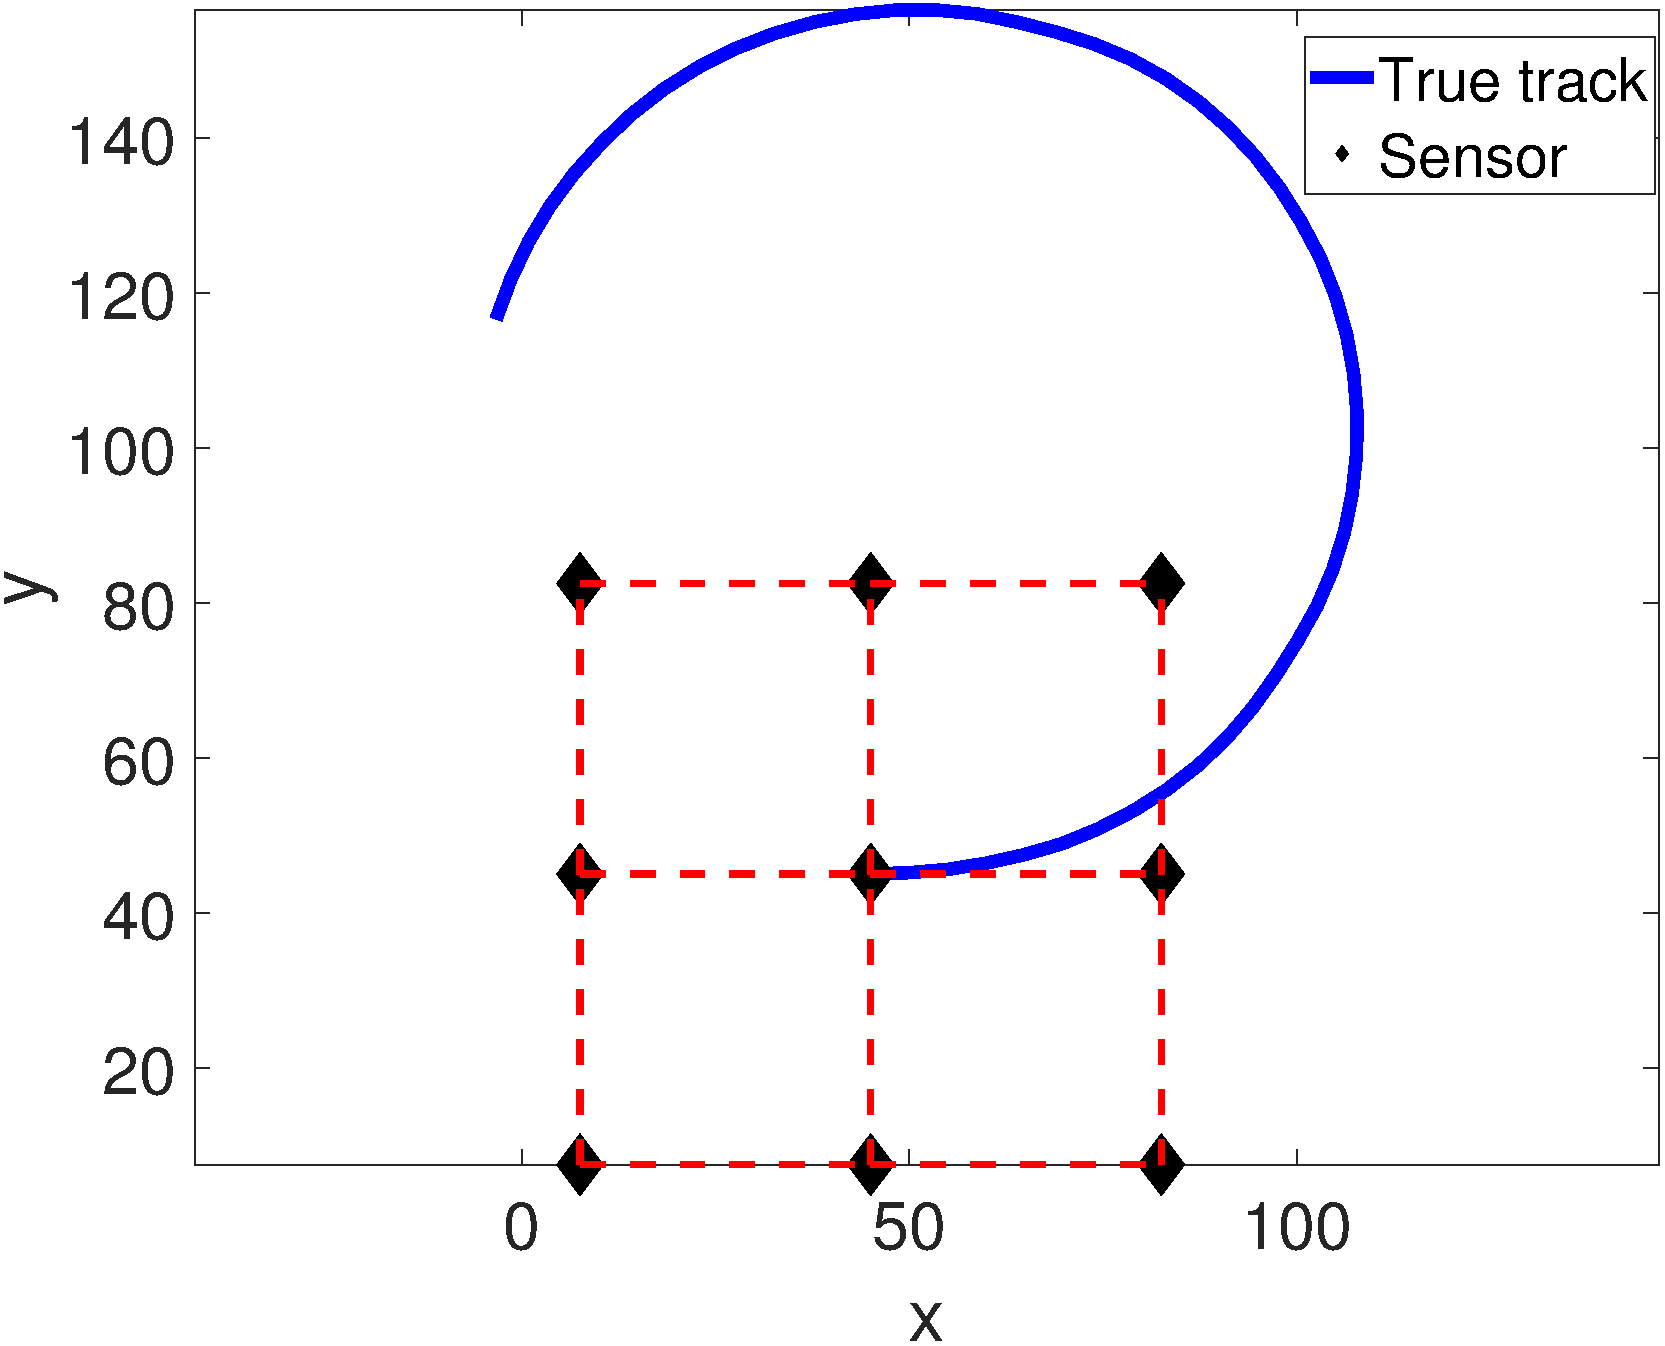
\includegraphics[width=0.65\textwidth]{Figures/track}
\caption{Target trajectory (blue curve) and sensor positions (red diamond)}
\label{fig:track}
\end{figure}

\subsection{Algorithm setup}
All particle filters use a total of $N=1000$ particles. At time step 1, we generate the initial particles using the true target state: $X_i(1) \sim \mathcal{N}(X(1), R_{\text{initial}})$ with $R_{\text{initial}}=\text{diag}([0.5^2,0.5^2,0.05^2,0.05^2])$. 

For LCpf, we use a set of basis functions involving all permutations of $x_t^iy_t^j$ with $0\leq i, j \leq d$ where $d$ is some user-specified max degree. For $d=2$, the basis functions would be
\begin{align*}
\beta_1(X) &= x_t^0 y_t^0 = 1 \\
\beta_2(X) &= x_t^0 y_t^1 = y_t \\
\beta_3(X) &= x_t^0 y_t^2 = y_t^2 \\
\beta_4(X) &= x_t^1 y_t^0 = x_t \\
... \\
\beta_9(X) &= x_t^2 y_t^2 
\end{align*}

For LApf, we construct a $K$-nearest neighbor graph and retain $m< N$ Eigenvectors as the basis of Laplacian transformation. For Clusterpf, all particles are grouped into $C$ clusters and a $K$-nearest neighbor graph is constructed to recover individual particle weights. 

Finally, the random number generators are synchronized to ensure that the particles remain the same across sensors. All summations are computed exactly without using any distributed algorithms. This ensures that no performance degradation is caused by consensus.

\subsection{Individual algorithm performance}
In this section, we evaluate the performance of individual algorithms with respect to their specific parameters. We run a number of Monte Carlo simulations on each algorithm while varying one single parameter. The track remains the same in each trial; but the measurements differ. 

We evaluate the algorithms' performances using two criterion: \textit{root mean squared error} (RMSE) of position estimate and total runtime (from initialization to end of time step 50). Our objective is to select a set of parameters that offer optimal trade-off between tracking performance and computational load. 

\subsubsection{Likelihood consensus particle filter}
Consider first LCpf. The max degree $d$ should offer a trade-off between tracking performance and total runtime. Higher degree $d$ leads to more basis functions and likely better approximation of the measurement model. On the other hand, more basis functions lead to more computation and longer runtime. 

\begin{figure}
\centering
\begin{subfigure}[RMSE]
{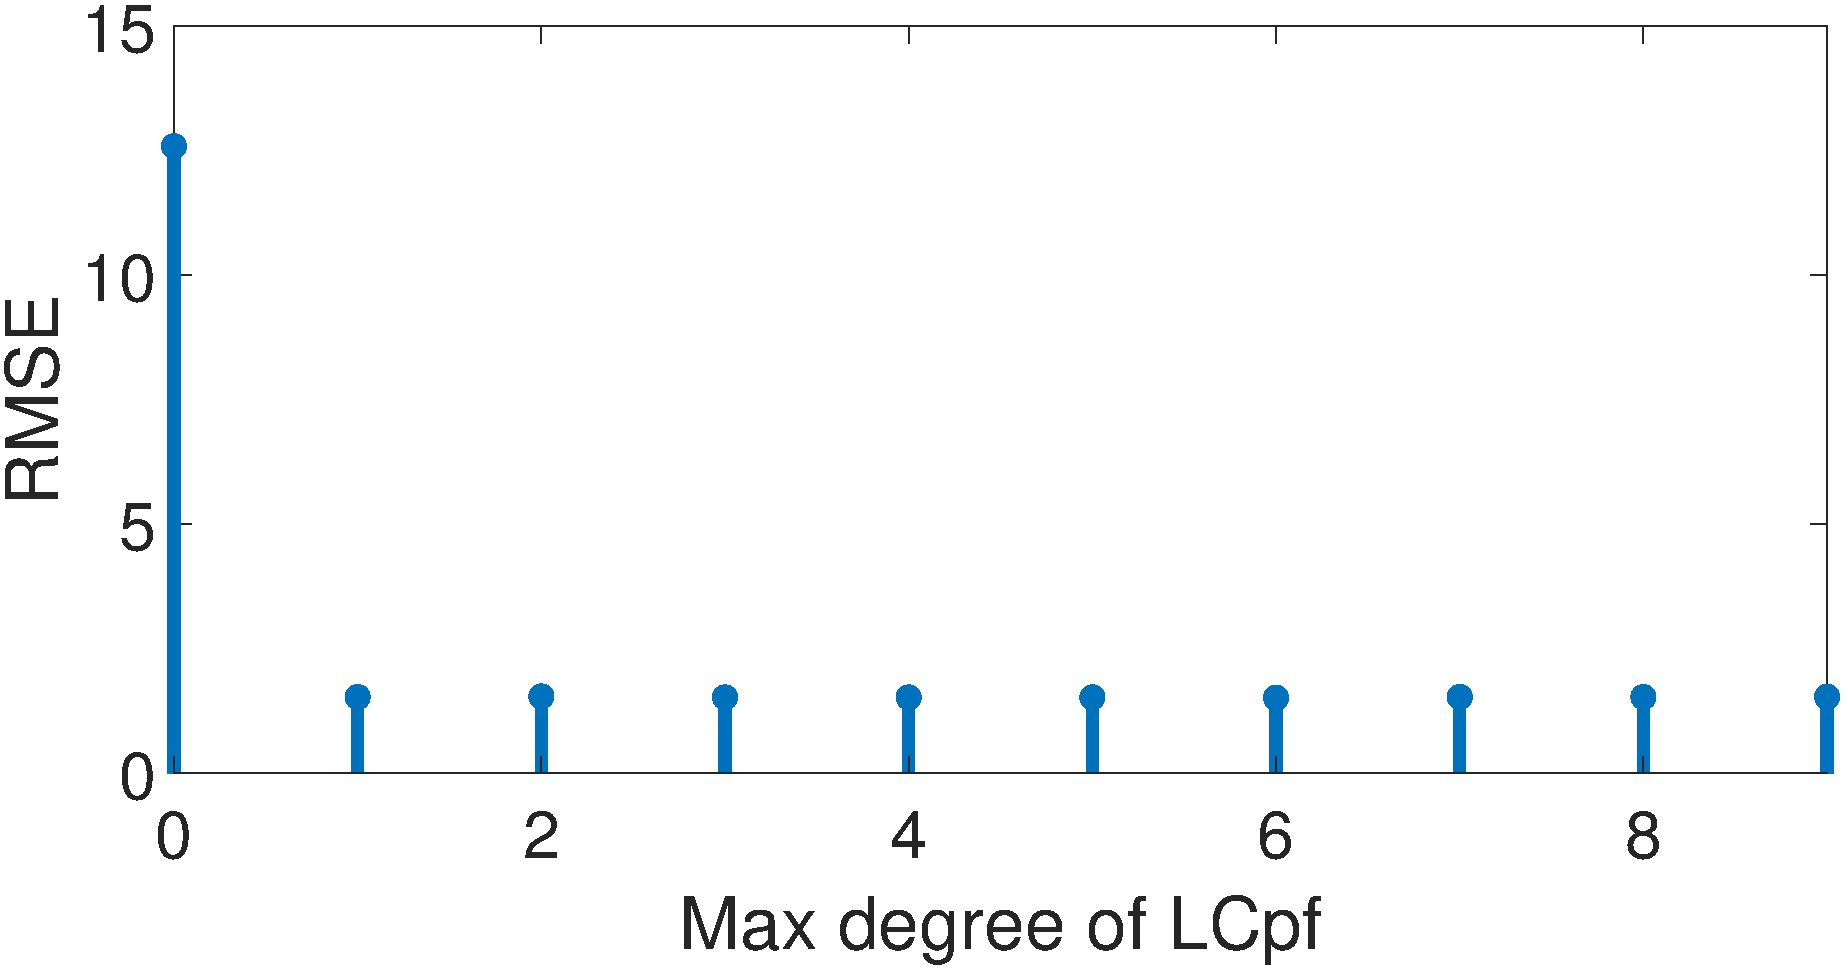
\includegraphics[width=0.49\textwidth]{Figures/RMSE_maxDegree}}
\end{subfigure}
\begin{subfigure}[total runtime]
{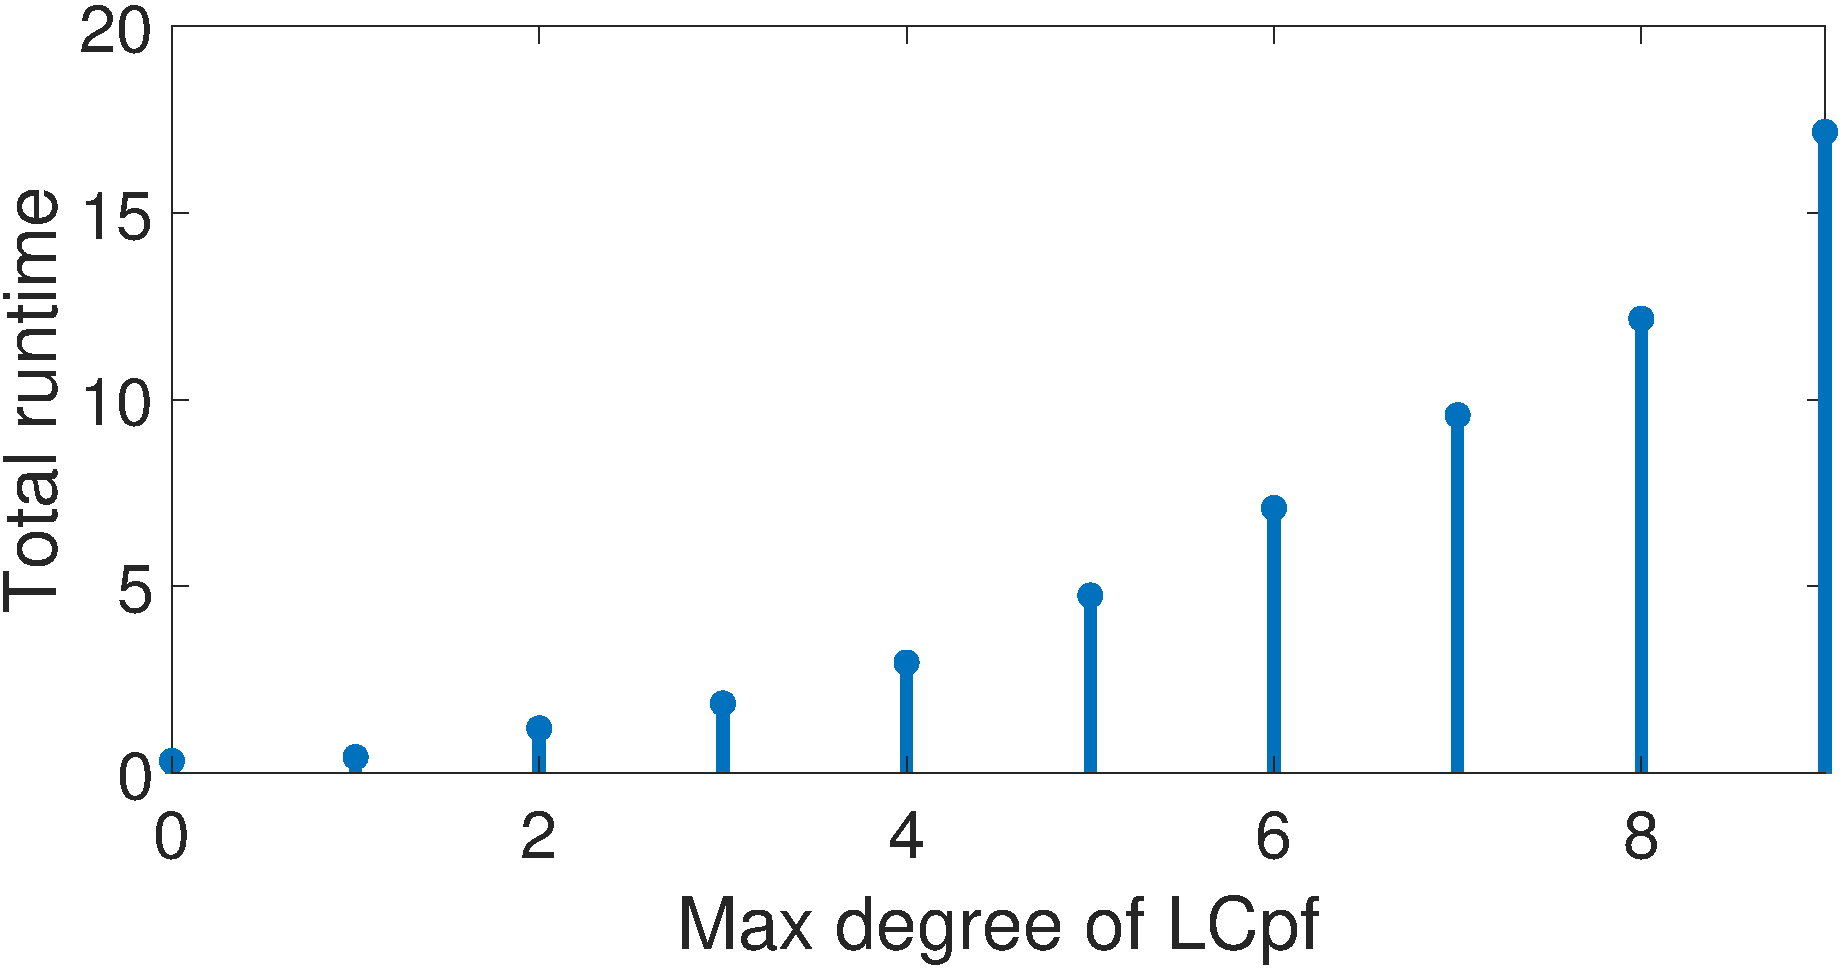
\includegraphics[width=0.49\textwidth]{Figures/runtime_maxDegree}}
\end{subfigure}
\caption{Boxplot of RMSE and runtime of LCpf with respect to max degree for 100 Monte Carlo trials. The red solid line in the subfig a is the average RMSE of BSpf for comparison.}
\label{fig:results_maxDegree}
\end{figure}

Fig.~\ref{fig:results_maxDegree} shows the boxplot of time-averaged RMSE and total runtime over 100 Monte Carlo trials. The total runtime increases with larger max degree as expected. On the other hand, we do not see any significant difference in RMSE for $1\leq d \leq 9$. This suggests that the additional basis functions for $d>1$ do not yield a better approximation of the measurement model $H(X_i)$. 

\begin{figure}
\centering
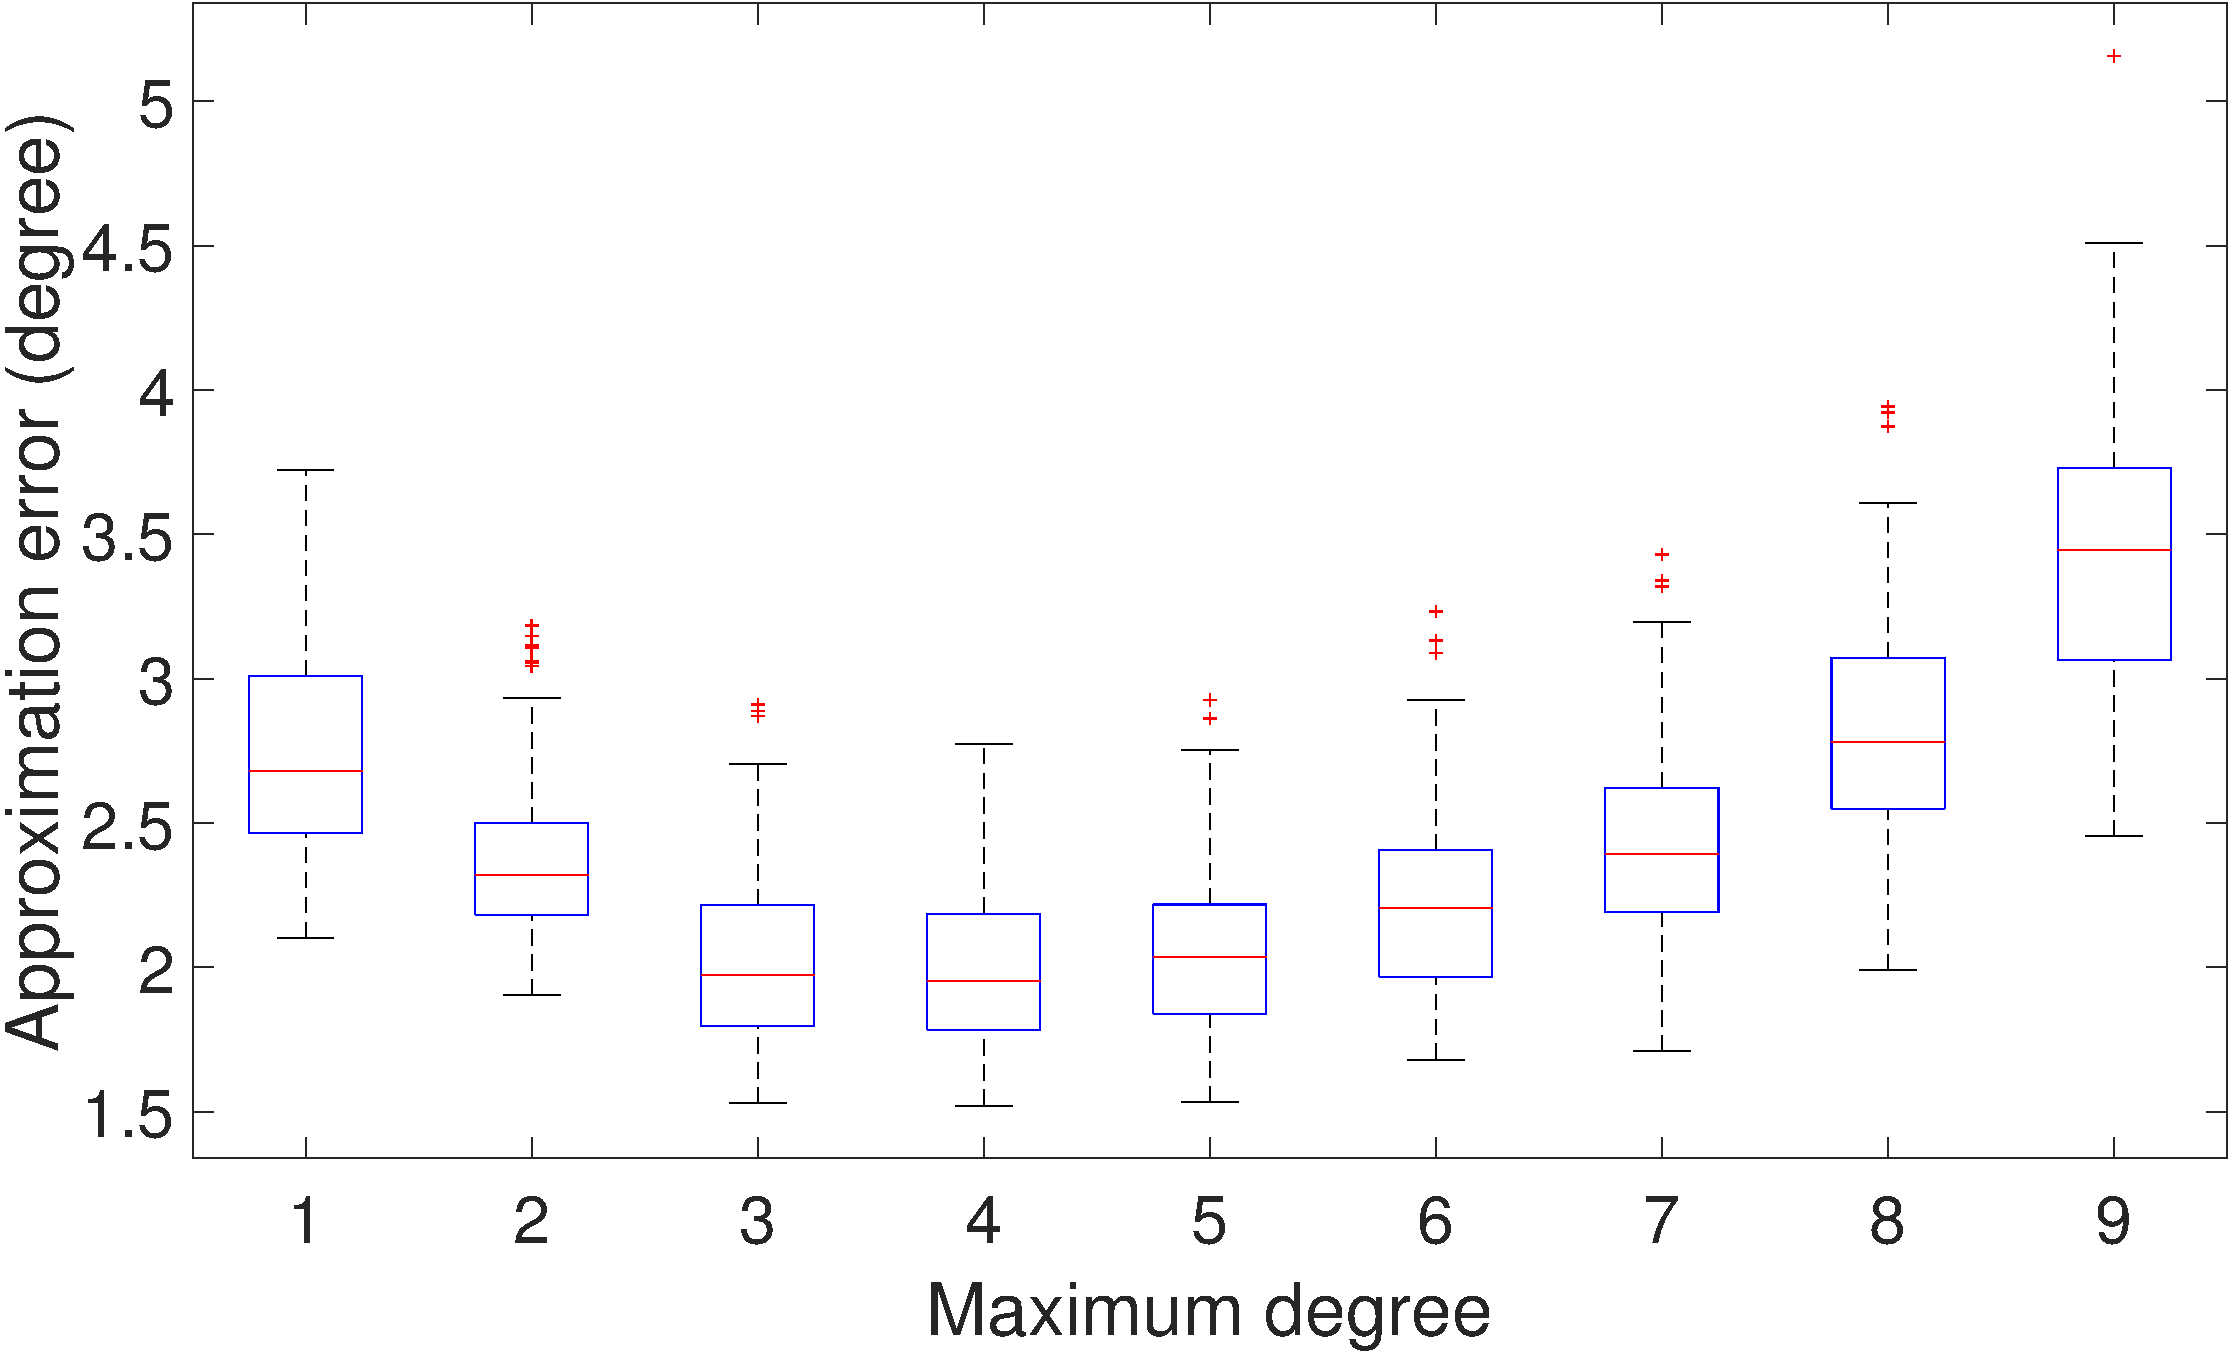
\includegraphics[width=0.55\textwidth]{Figures/LCpf_approx_error.pdf}
\label{fig:LCpf_approx_error}
\caption{Boxplot of measurement approximation error with respect to max degree. All results are computed over 100 Monte Carlo trials}
\end{figure}

To verify our conjecture, we compute the following metric. At each time step, we compute the aggregate approximation error over all $S$ measurements for each particle ($\sum_{s=1}^S H_s(X_i)-\hat(H)_s(X_i)$), and report the average value $\sum_{i=1}^N \sum_{s=1}^S(H_s(X_i)-\hat(H)_s(X_i))/N$. 

Fig.~\ref{fig:LCpf_approx_error} shows that the approximation error with respect to max degree. The approximation error decreases until $d=4$ and increases afterwards; but the difference is rather small with a maximum difference of 1.5 degree (versus the 5 degrees standard deviation of measurement noise). This small difference in approximation error directly translates to negligible difference in tracking performance. Based on the computational overhead, we will select $d=1$ for LCpf in subsequent simulations. 

\subsubsection{Laplacian approximation particle filter}
The LApf has two parameters of interest: $K$, the number of nearest neighbors for the particle graph, and $m$, the number of Eigenvectors for the transformation. Different values of $K$ yield different graphs over the same particles and by extension different Eigenvectors. Retaining more Eigenvectors yields a better approximation of particle log-likelihoods at the cost of higher computation overhead. 

Table.~\ref{tab:RMSE_LApf} shows the average RMSE of LApf with respect to $K$ and $m$. As $m$ increases, the RMSE tends to decrease as expected since the approximation error is reduced.   At $m=1000$, there is no approximation error and the RMSE is constant for all values $K$ and on-par with that of centralized BSpf. For $m=6, 10, 20$, we see a decrease in RMSE as $K$ goes up.  For $m= 100, 200, 500$, the RMSE has small fluctuations over $K$. 

To understand these trends, we compute and report at each time step the approximation error of normalized particle weights: $\sqrt{\sum_{i=1}^N (w_i-\hat{w}_i)^2}$ where $w_i$ is the exact particle weight and $\hat{w}_i$ is the approximate value using $m$ eigenvectors. Table.~\ref{tab:Approx_error_LApf} shows the results. As expected, at $m=1000$, there is no approximation error as all eigenvectors are used. For small values of $m$, we see a drastic decrease in approximation error as $K$ increases. This in turn translates to lower RMSE. For $m\geq 100$, the approximation error actually goes up with as $K$ increases. It is worth noting that the high values of $m$ ensure the approximation error remains small. 

\begin{table}[h!]
\centering
\begin{tabular}{|l|l|l|l|l|l|l|l|}
\hline
        & m = 6  & 10     & 20     & 100    & 200    & 500    & 1000   \\ \hline
K = 3   & 5.4804 & 4.4057 & 3.9159 & 2.1505 & 2.1612 & 2.2161 & 2.1646 \\ \hline
4       & 4.2176 & 3.8376 & 3.6131 & 2.2138 & 2.195  & 2.2501 & 2.1646 \\ \hline
5       & 4.3284 & 3.6929 & 2.914  & 2.1928 & 2.2302 & 2.2292 & 2.1646 \\ \hline
6       & 4.1016 & 3.3112 & 2.3407 & 2.2309 & 2.233  & 2.2877 & 2.1646 \\ \hline
7       & 3.6605 & 2.8502 & 2.2711 & 2.1899 & 2.229  & 2.2864 & 2.1646 \\ \hline
8       & 3.436  & 2.3306 & 2.1202 & 2.1923 & 2.235  & 2.2655 & 2.1646 \\ \hline
9       & 3.1273 & 2.2126 & 2.1998 & 2.2885 & 2.2476 & 2.2789 & 2.1646 \\ \hline
10      & 2.9664 & 2.231  & 2.0918 & 2.1727 & 2.2219 & 2.2215 & 2.1646 \\ \hline
20      & 2.5182 & 2.1113 & 2.1180 & 2.3057 & 2.2763 & 2.2745    & 2.1646 \\ \hline
50      & 2.2559 & 2.0106 & 2.1037 & 2.2813 & 2.3008 & 2.2571    & 2.1646 \\ \hline
100     & 2.2783 & 2.2772 & 2.3185 & 2.2922 & 2.2950 & 2.3043    & 2.1646 \\ \hline
\end{tabular}
\caption{RMSE of LApf with respect to $m$ and $K$ over 100 Monte Carlo trials}
\label{tab:RMSE_LApf}
\end{table}

\begin{table}[h!]
\centering
\begin{tabular}{|l|l|l|l|l|l|l|l|}
\hline
        & m = 6  & 10     & 20     & 100    & 200    & 500    & 1000 \\ \hline
KNN = 3 & 0.0747 & 0.0589 & 0.0456 & 0.0102 & 0.0088 & 0.0096 & 0    \\ \hline
4       & 0.0477 & 0.0408 & 0.0328 & 0.0109 & 0.0115 & 0.0113 & 0    \\ \hline
5       & 0.0386 & 0.0329 & 0.0221 & 0.0127 & 0.0121 & 0.0118 & 0    \\ \hline
6       & 0.0341 & 0.0245 & 0.0173 & 0.0129 & 0.0143 & 0.0137 & 0    \\ \hline
7       & 0.0279 & 0.021  & 0.0146 & 0.0126 & 0.016  & 0.0137 & 0    \\ \hline
8       & 0.0248 & 0.0183 & 0.0141 & 0.0137 & 0.0166 & 0.014  & 0    \\ \hline
9       & 0.0242 & 0.0171 & 0.0139 & 0.0155 & 0.016  & 0.0144 & 0    \\ \hline
10      & 0.0224 & 0.0159 & 0.0141 & 0.014  & 0.0165 & 0.0149 & 0    \\ \hline
20      & 0.0186 & 0.0166 & 0.0150 & 0.0200 & 0.0191 & 0.0174         & 0    \\ \hline
50      & 0.0193 & 0.0170 & 0.0199 & 0.0214 & 0.0213 & 0.0195         & 0    \\ \hline
100     & 0.0209 & 0.0223 & 0.0252 & 0.0249 & 0.0230 & 0.0214         & 0 \\ \hline
\end{tabular}
\caption{Approximation error of LApf with respect to $m$ and $K$ over 100 Monte Carlo trials}
\label{tab:Approx_error_LApf}
\end{table}

Table.~\ref{tab:runtime_LApf} shows the total runtime of LApf with respect to $K$ and $m$. For $1\leq K \leq 10$, when $m$ increases, the particle log-likelihoods are encoded using more coefficients. However, since this is a matrix multiplication operation, the difference in computational overhead is negligible and there is no significant variation in computational overhead. For $K=20, 50, 100$, surprisingly, there is a significant fluctuation in runtime as $m$ increases. On the other hand, at $K=7$, there is a huge spike in runtime for all values of $m$. Fig.~\ref{fig:time_bar_LApf} shows the breakdown of total runtime for $m=10$. It appears that the computational overhead of eigenvalue decomposition spikes at $K=7$. It is not yet clear what causes this sudden spike. We omit the figures for other values of $m$ to save space; but it is worth nothing that the eigenvalue decomposition accounts for the overwhelming majority of computational overhead in all cases. 

\begin{table}[h!]
\centering
\begin{tabular}{|l|l|l|l|l|l|l|l|}
\hline
      & m = 6   & 10      & 20      & 100     & 200     & 500     & 1000    \\ \hline
K = 3 & 46.621  & 45.8677 & 44.6806 & 47.9622 & 47.4402 & 47.213  & 47.9443 \\ \hline
4     & 47.61   & 45.8321 & 46.9099 & 44.1239 & 46.8175 & 45.7268 & 48.0369 \\ \hline
5     & 45.5334 & 45.9404 & 44.9823 & 44.2019 & 47.1917 & 46.8049 & 49.0212 \\ \hline
6     & 47.1295 & 48.5234 & 47.4019 & 49.2646 & 50.1962 & 54.1456 & 58.088  \\ \hline
7     & 59.0893 & 56.0343 & 58.6746 & 56.3333 & 58.1322 & 55.1389 & 49.3091 \\ \hline
8     & 48.8316 & 47.9977 & 47.1873 & 45.6619 & 46.6635 & 47.3256 & 48.1953 \\ \hline
9     & 49.4382 & 51.4236 & 48.8129 & 46.9926 & 47.2865 & 51.273  & 57.2445 \\ \hline
10    & 46.4701 & 46.178  & 49.3883 & 50.8106 & 51.7062 & 49.7496 & 47.8554 \\ \hline
20    & 45.1474 & 48.0359 & 42.6048 & 29.7810 & 31.1612 & 30.2740 & 30.4691 \\ \hline
50    & 47.3068 & 53.4298 & 39.3070 & 31.5229 & 31.4748 & 31.1005 & 35.6691 \\ \hline
100   & 55.7847 & 44.9831 & 39.8943 & 36.4267 & 32.4495 & 33.2130 & 34.6833 \\ \hline
\end{tabular}
\caption{Total runtime of LApf with respect to $m$ and $K$ over 100 Monte Carlo trials}
\label{tab:runtime_LApf}
\end{table}

\begin{figure}
\centering
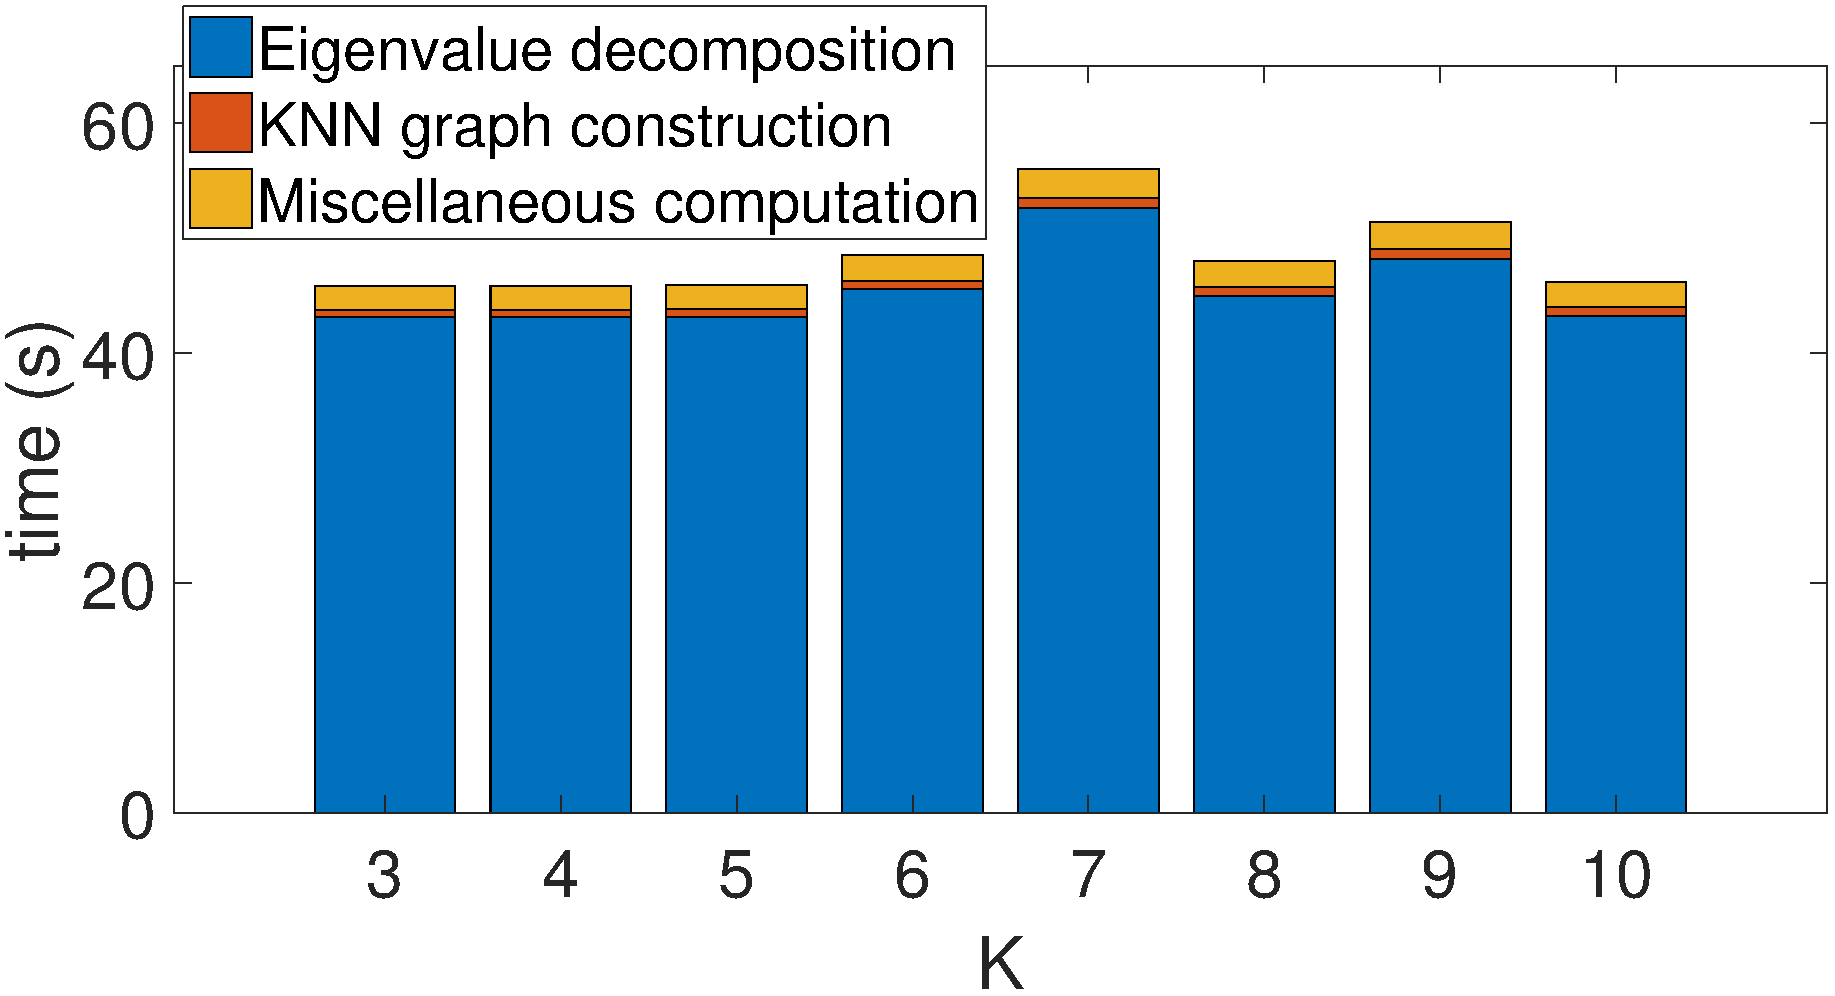
\includegraphics[width=0.75\textwidth]{Figures/time_bar_LApf.pdf}
\caption{Breakdown of total runtime of LApf with respect to $K$ for $m=10$}
\label{fig:time_bar_LApf}
\end{figure}

%Fig.~\ref{fig:RMSE_LApf_KNN} shows the average RMSE with respect to $K$ for different values of $m$. We also include the results of centralized BSpf as baseline. For $m=6$ (which requires the same amount of communication overhead as CSSpf), the RMSE decreases with increasing $K$. For $m=6$, the RMSE stops decreasing after $K=6$. For larger values of $m$, the approximation error of particle log-likelihoods would be low enough that the RMSE is fairly constant for all values of $K$. 
%
%\begin{figure}
%\centering
%\subfigure[$m$=6]{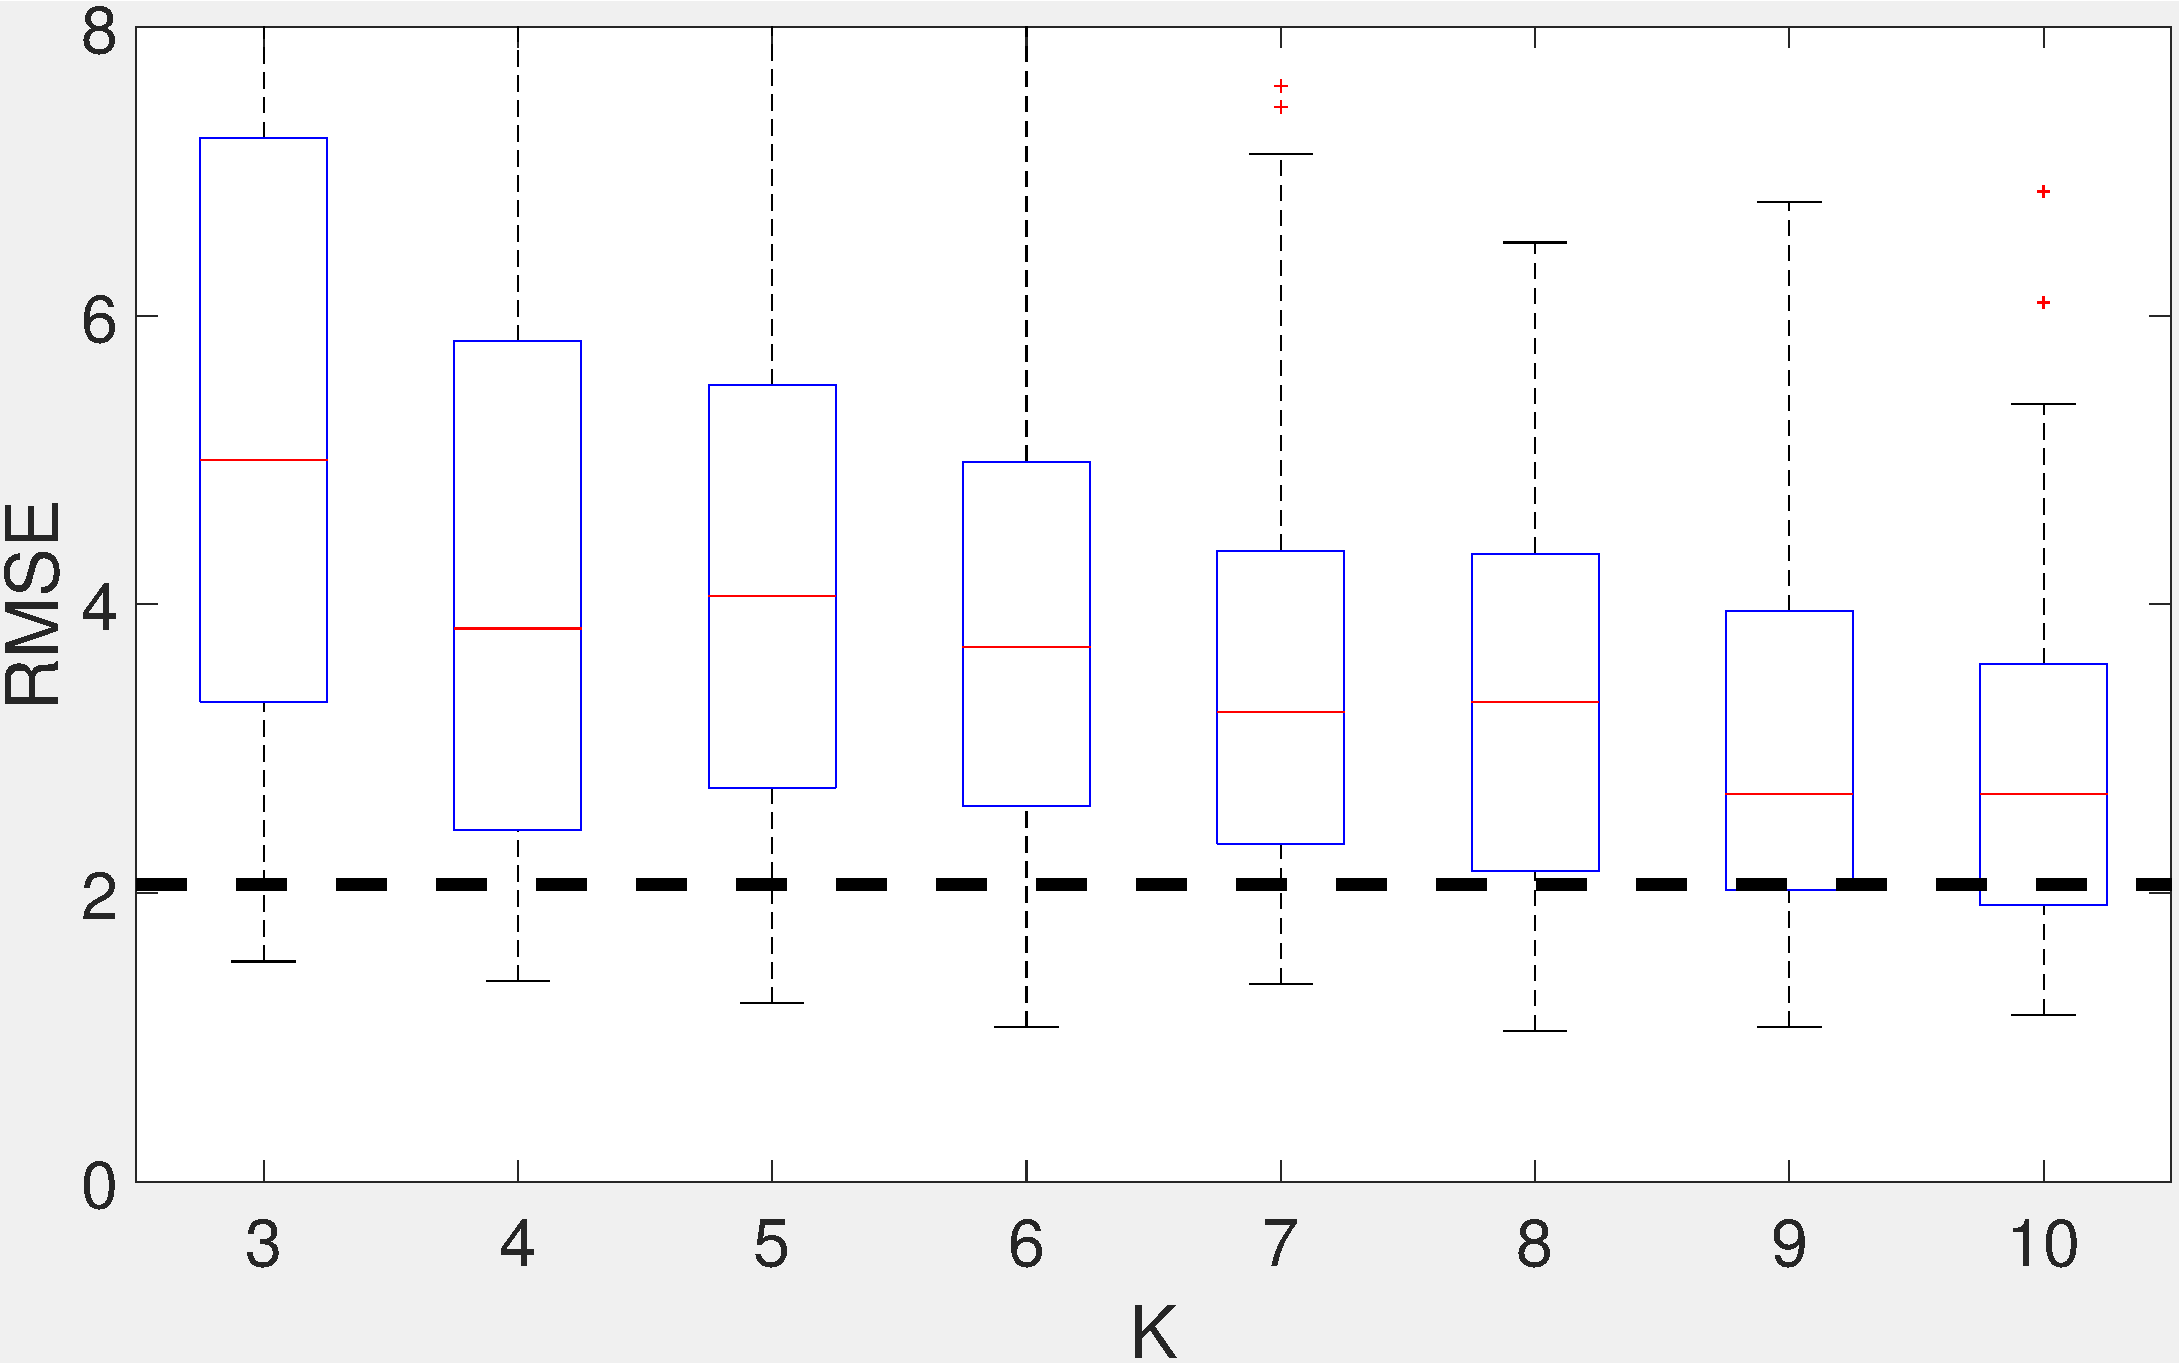
\includegraphics[width=0.45\textwidth]{Figures/RMSE_LApf_KNN_m6}}
%\subfigure[$m$=20]{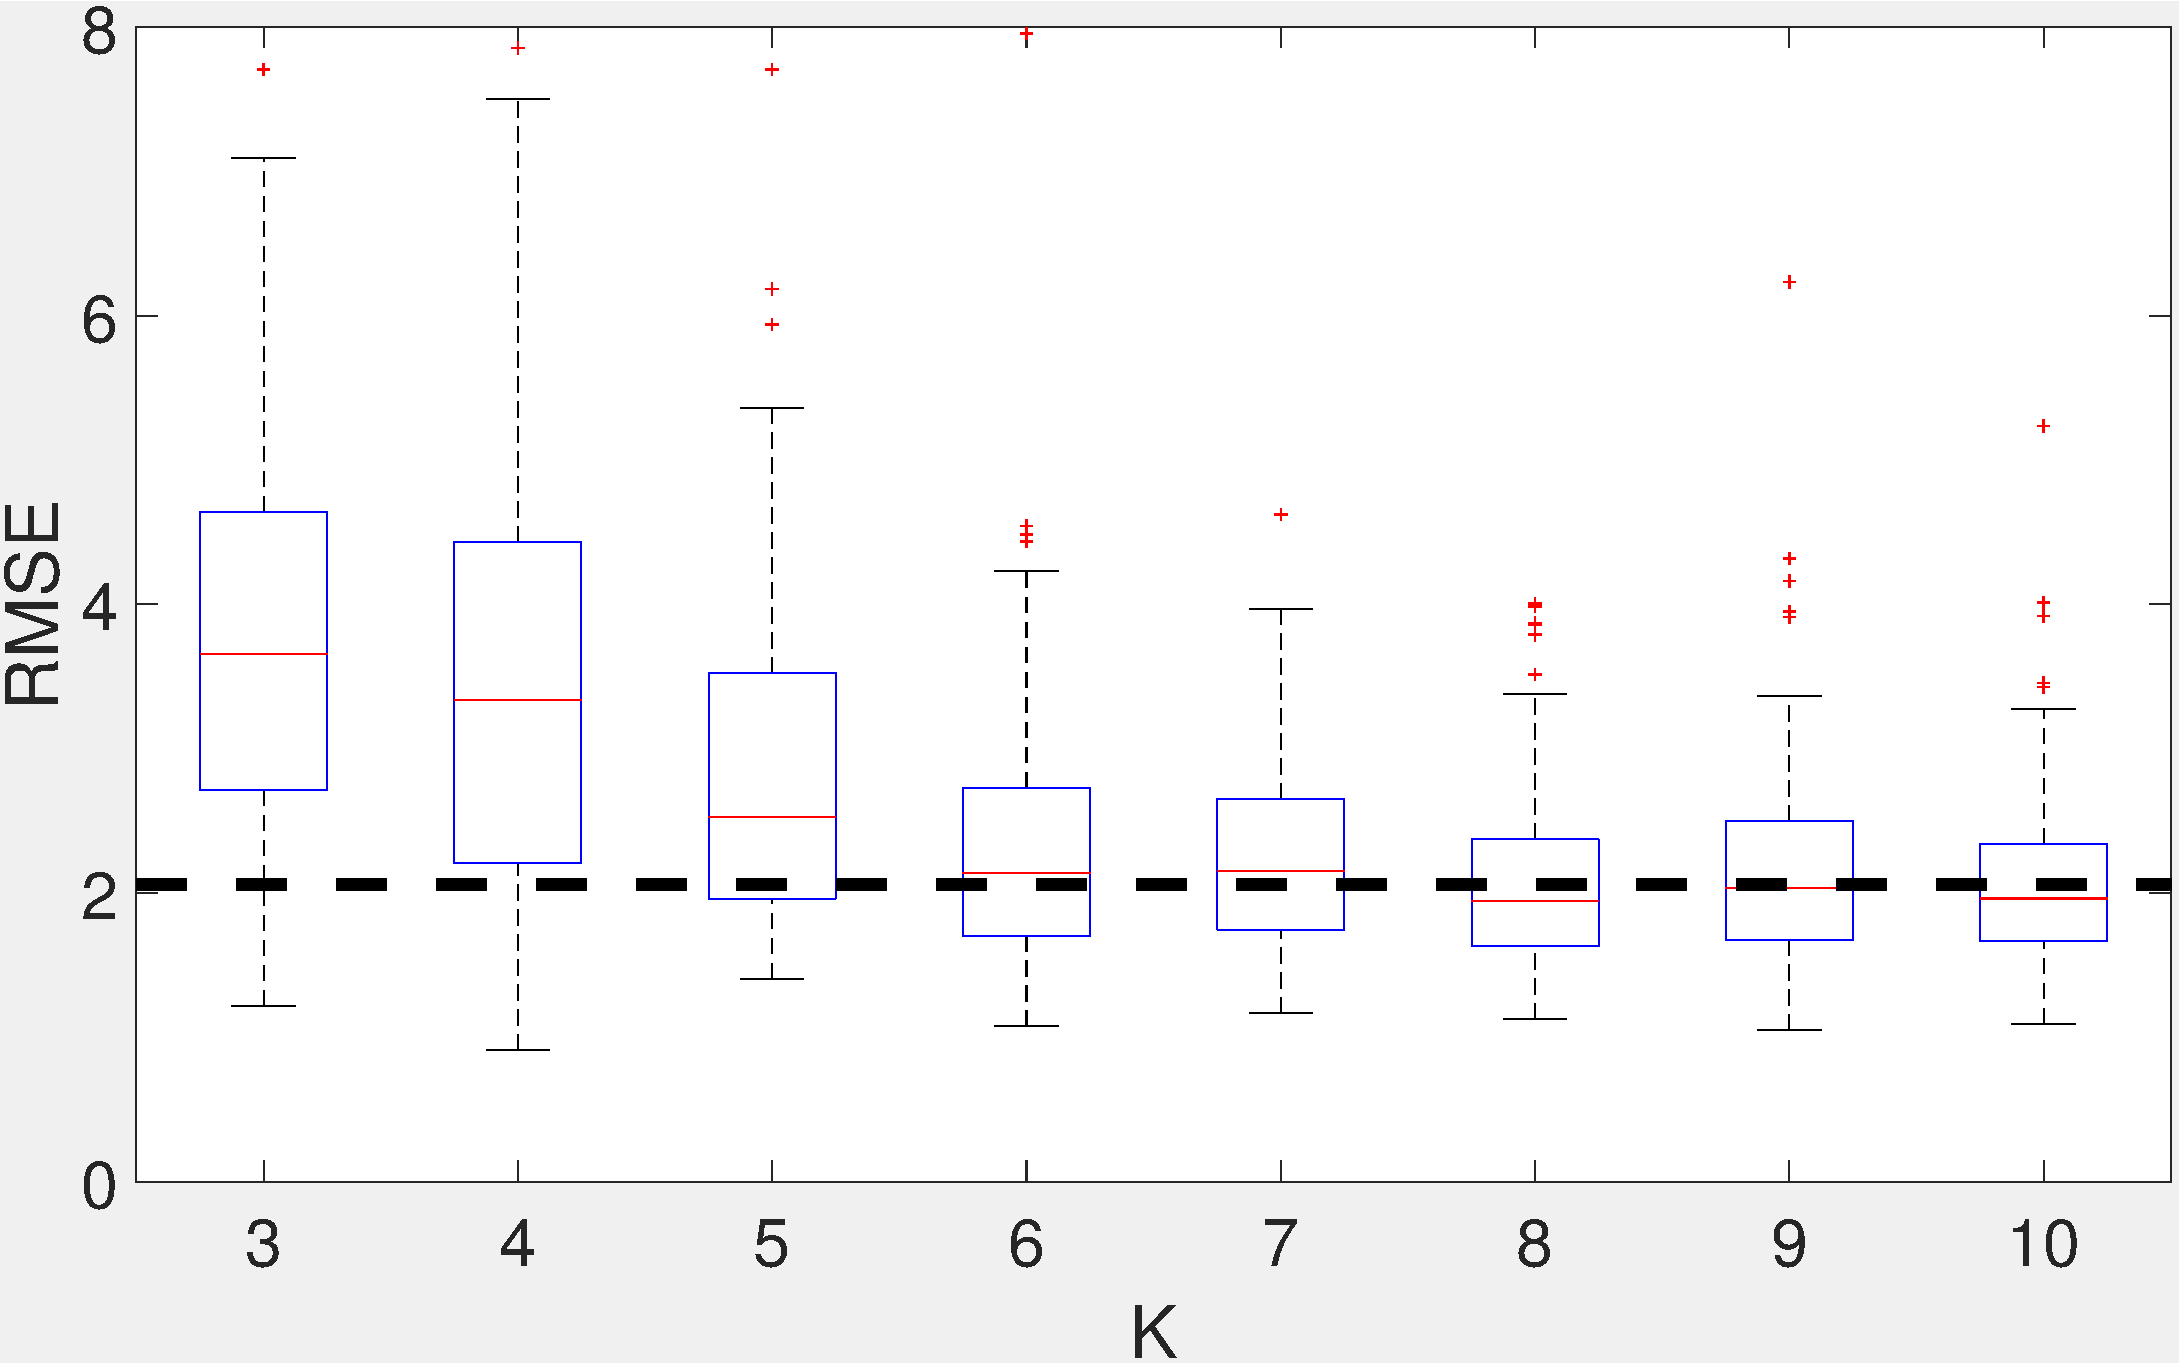
\includegraphics[width=0.45\textwidth]{Figures/RMSE_LApf_KNN_m20}}
%\subfigure[$m$=500]{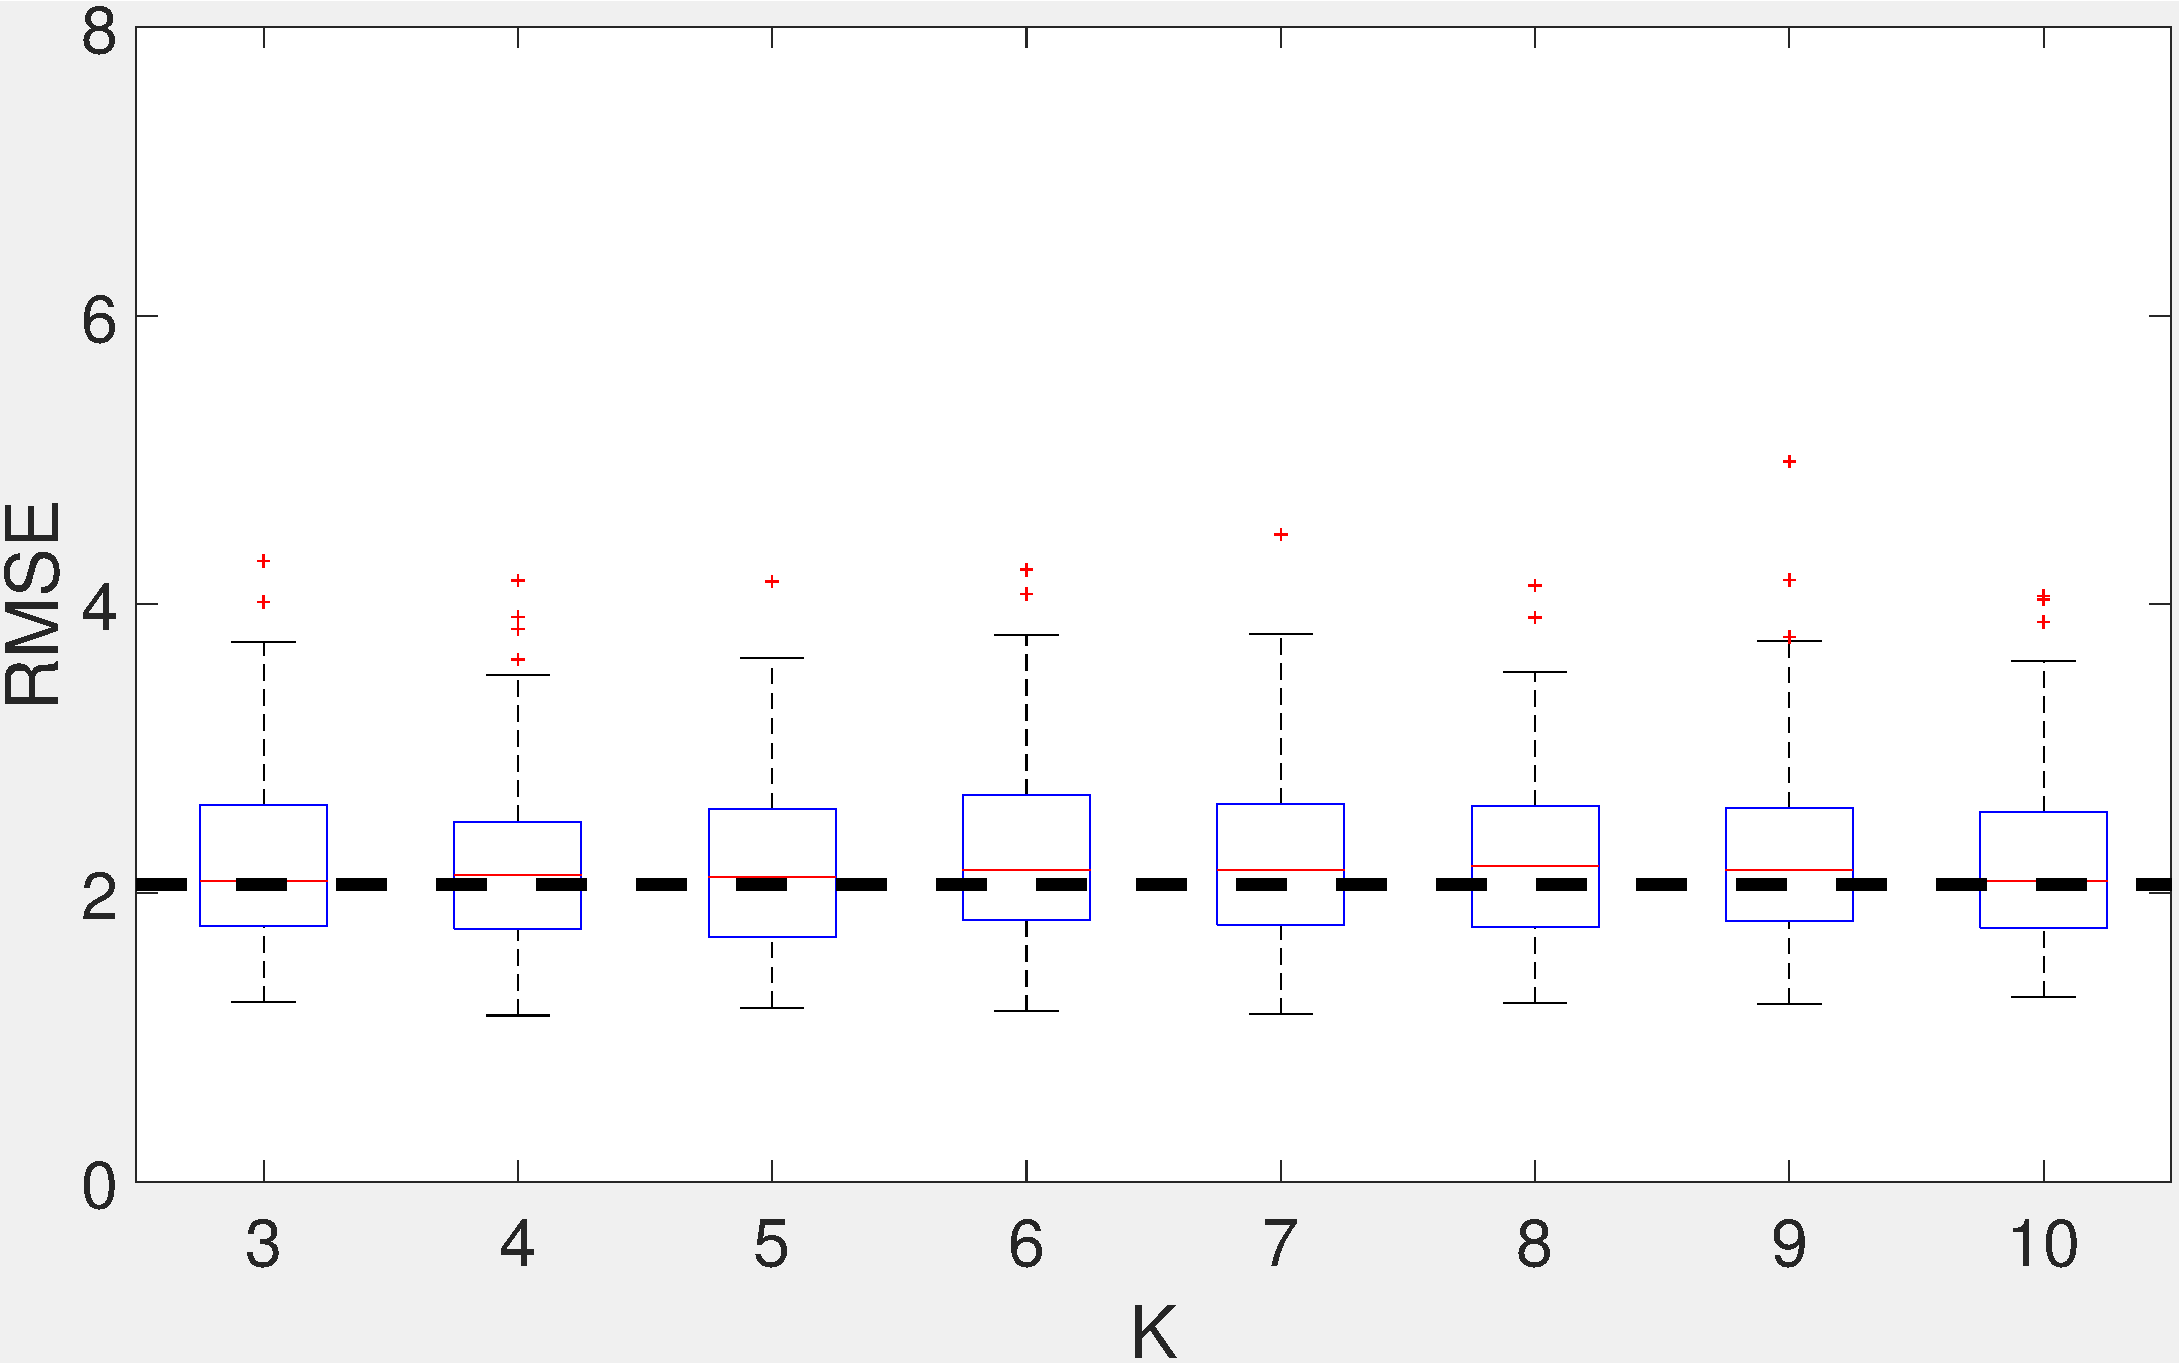
\includegraphics[width=0.45\textwidth]{Figures/RMSE_LApf_KNN_m500}}
%\subfigure[$m$=1000]{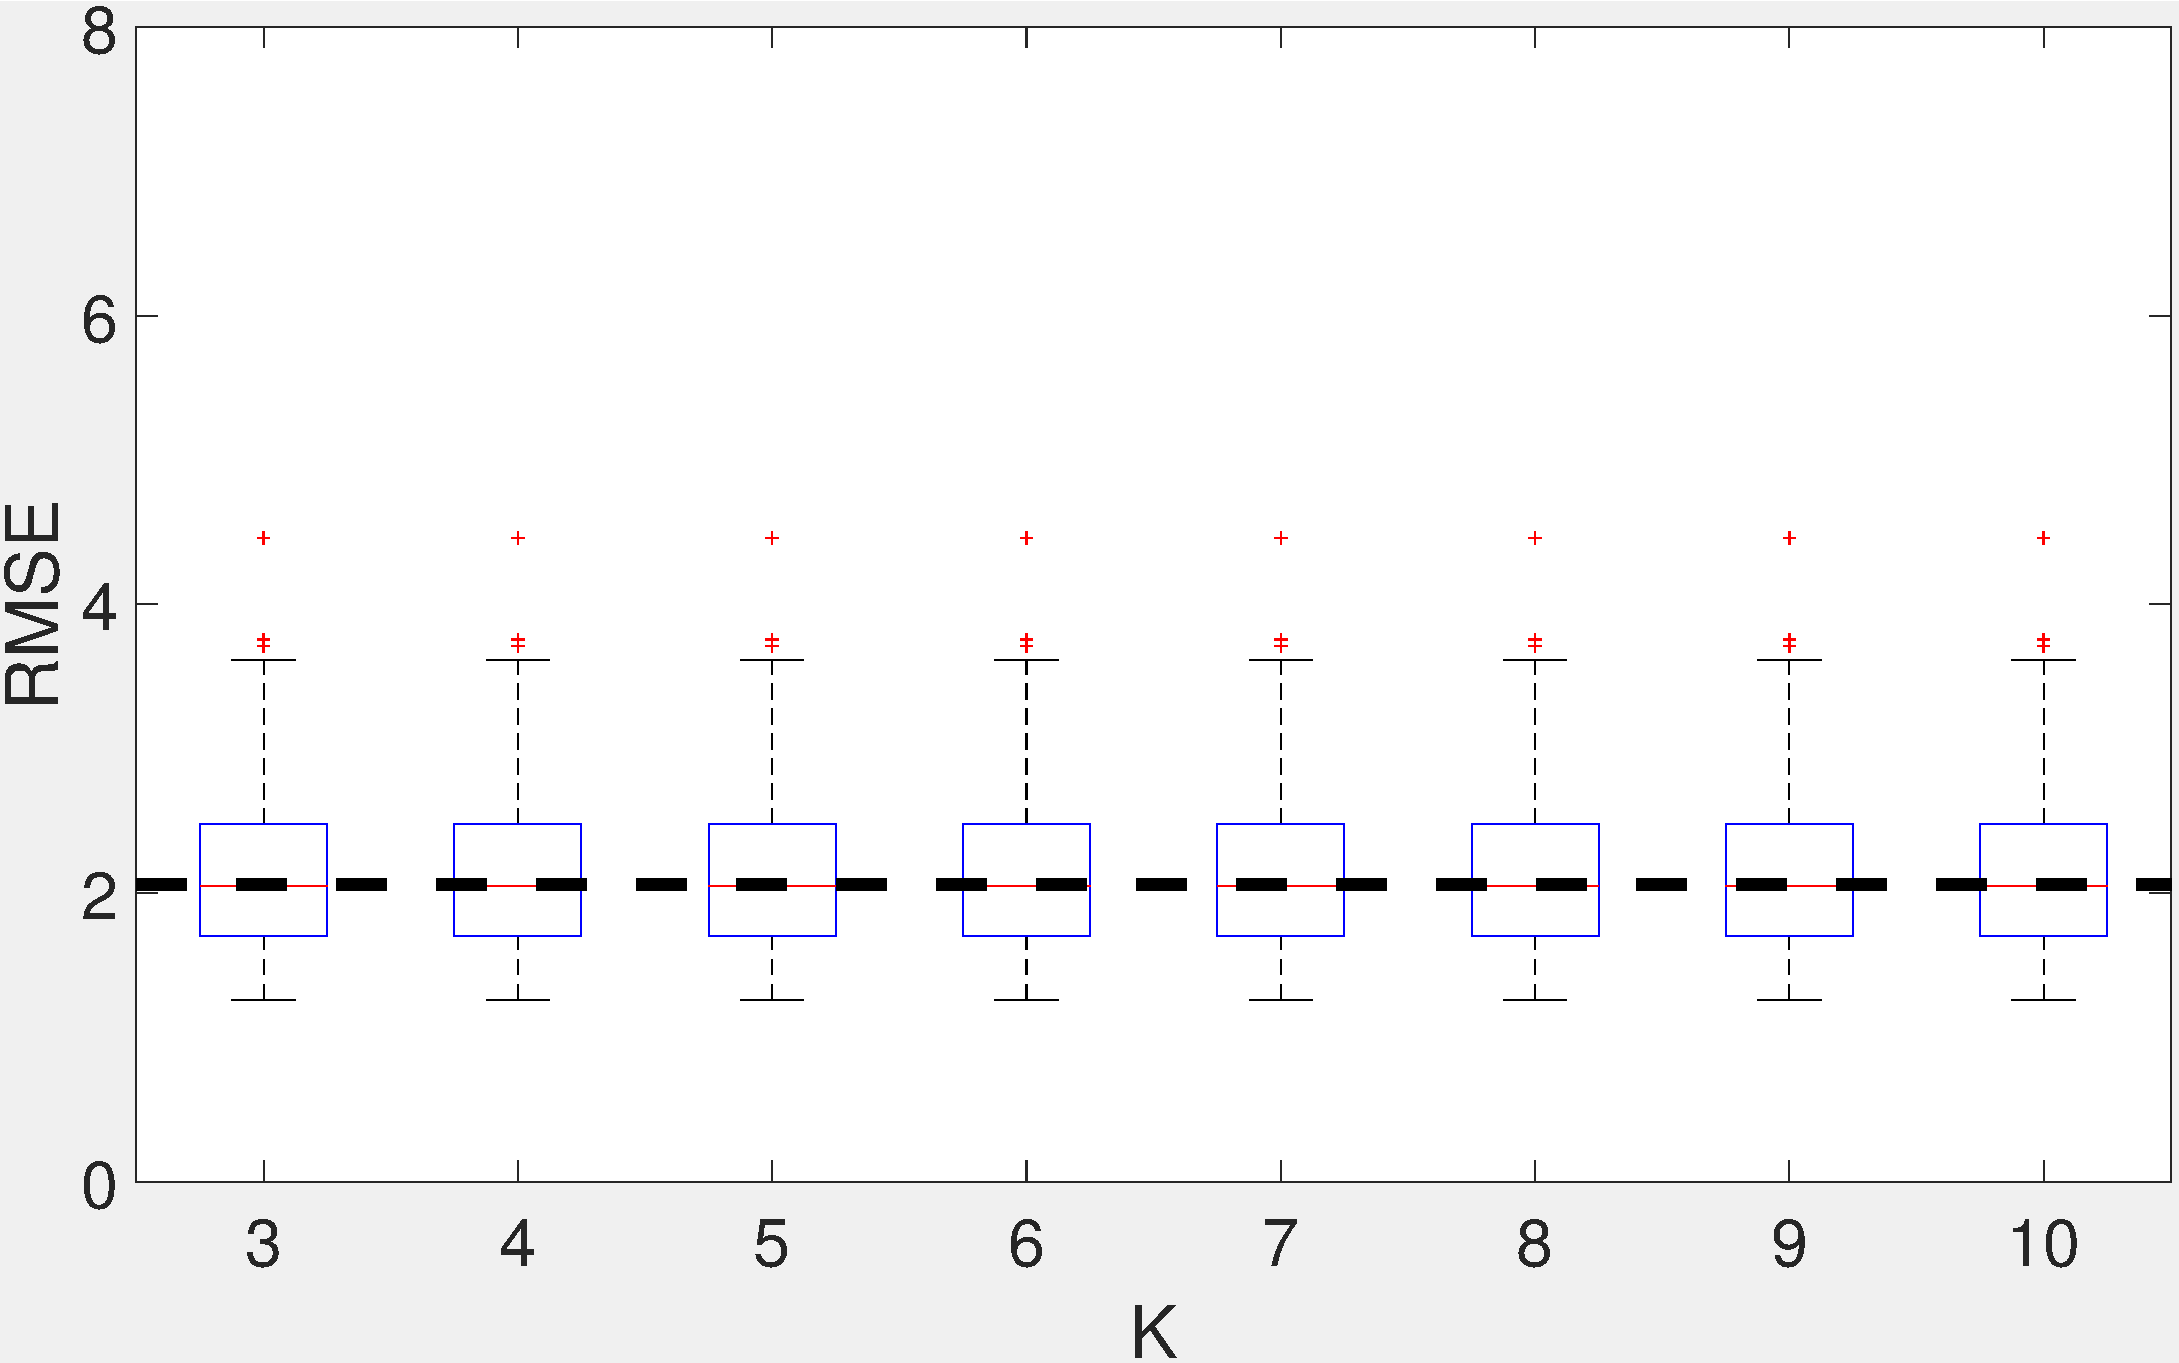
\includegraphics[width=0.45\textwidth]{Figures/RMSE_LApf_KNN_m1000}}
%\caption{Boxplot of time-averaged RMSE of LApf with respect to the number of eigenvectors over 100 Monte Carlo trials for different values of $K$.}
%\label{fig:RMSE_LApf_KNN}
%\end{figure}

%Table.~\ref{tab:time_LApf} shows the average total runtime with respect to $K$ for different values of $m$. 
%
%\begin{table}[H]
%\centering
%\begin{tabular}{|l|l|l|l|l|l|l|l|}
%\hline
%        & $m$ = 6   & 10      & 20      & 100     & 200     & 500     & 1000    \\ \hline
%$K$ = 3 & 46.621  & 45.8677 & 44.6806 & 47.9622 & 47.4402 & 47.213  & 47.9443 \\ \hline
%4       & 47.61   & 45.8321 & 46.9099 & 44.1239 & 46.8175 & 45.7268 & 48.0369 \\ \hline
%5       & 45.5334 & 45.9404 & 44.9823 & 44.2019 & 47.1917 & 46.8049 & 49.0212 \\ \hline
%6       & 47.1295 & 48.5234 & 47.4019 & 49.2646 & 50.1962 & 54.1456 & 58.088  \\ \hline
%7       & 59.0893 & 56.0343 & 58.6746 & 56.3333 & 58.1322 & 55.1389 & 49.3091 \\ \hline
%8       & 48.8316 & 47.9977 & 47.1873 & 45.6619 & 46.6635 & 47.3256 & 48.1953 \\ \hline
%9       & 49.4382 & 51.4236 & 48.8129 & 46.9926 & 47.2865 & 51.273  & 57.2445 \\ \hline
%10      & 46.4701 & 46.178  & 49.3883 & 50.8106 & 51.7062 & 49.7496 & 47.8554 \\ \hline
%\end{tabular}
%\caption{Total runtime of LApf with respect to $K$ and $m$. All results area averaged over 50 time steps and 100 Monte-Carlo trials.}
%\label{tab:time_LApf}
%\end{table}




\subsubsection{Cluster particle filter}
The Clusterpf has two parameters of interest: number of clusters $C$ and number of neighbors $K$ for the graph construction. Table~\ref{tab:RMSE_clusterpf} shows the average RMSE of Clusterpf with respect to $C$ and $K$. As $C$ increases, the RMSE decreases. At $C=N=1000$, the Clusterpf is equivalent to the centralized BSpf (assuming distributed summation without error) and the performance is independent of $K$. For any given value of $C$, as $K$ increases, RMSE decreases. Higher value of $C$ requires higher communication overhead whereas the higher $K$ generates a more connected graph with more computational overhead. This suggests that one may opt for a higher value of $K$ in exchange for reduced communication overhead. 

\begin{table}[h!]
\centering
\begin{tabular}{|l|l|l|l|l|l|l|l|l|}
\hline
      & C = 6  & 10     & 20     & 50     & 100    & 200    & 500    & 1000  \\ \hline
K = 3 & 7.2659 & 5.8947 & 4.9396 & 4.2876 & 3.5259 & 2.9242 & 2.1867 & 2.145 \\ \hline
4     & 5.788  & 4.8958 & 4.2774 & 3.8178 & 3.6676 & 2.7393 & 2.1351 & 2.145 \\ \hline
5     & 4.8997 & 4.3572 & 4.2338 & 3.6465 & 3.3935 & 2.6175 & 2.082  & 2.145 \\ \hline
6     & 4.484  & 3.5367 & 3.4824 & 3.3628 & 2.9538 & 2.3805 & 2.2021 & 2.145 \\ \hline
7     & 3.8512 & 3.8754 & 3.7534 & 3.2243 & 2.6819 & 2.2898 & 2.1499 & 2.145 \\ \hline
8     & 3.9089 & 3.3702 & 3.3426 & 2.9276 & 2.5027 & 2.2326 & 2.1574 & 2.145 \\ \hline
9     & 3.5868 & 3.1086 & 3.0701 & 2.8636 & 2.5661 & 2.2189 & 2.161  & 2.145 \\ \hline
10    & 3.51   & 3.0733 & 2.919  & 2.4383 & 2.3067 & 2.1811 & 2.1323 & 2.145 \\ \hline
20    & 2.4083 & 2.2209 & 2.2114 & 2.2414 & 2.2362 & 2.2464 & 2.1979 & 2.145 \\ \hline
50    & 2.2432 & 2.2315 & 2.1922 & 2.274  & 2.2721 & 2.2163 & 2.2494 & 2.145 \\ \hline
100   & 2.3841 & 2.2779 & 2.2087 & 2.1232 & 2.1998 & 2.2225 & 2.233  & 2.145 \\ \hline
\end{tabular}
\caption{RMSE of Clusterpf with respect to $K$ and $C$ over 100 Monte Carlo trials}
\label{tab:RMSE_clusterpf}
\end{table}

Table.~\ref{tab:runtime_Clusterpf} shows the total runtime of Clusterpf with respect to $K$ and $m$. As $C$ increases, so does the runtime with a huge spike after $C=200$. A detailed breakdown of total runtime shows that clustering of particles is the sole cause of high runtime (i.e., clustering particles requires more than 10 minutes for $C=1000$). For a given value of $C$, increasing $K$ leads to higher runtime which is caused by the higher computational overhead for nearest-neighbor graph construction. 

\begin{table}[h!]
\centering
\begin{tabular}{|l|l|l|l|l|l|l|l|l|}
\hline
      & C = 6   & 10      & 20      & 50      & 100     & 200     & 500      & 1000     \\ \hline
K = 3 & 7.5892  & 7.261   & 7.319   & 11.6321 & 19.1915 & 42.2104 & 194.2847 & 748.8655 \\ \hline
4     & 5.3822  & 7.376   & 8.1377  & 10.3778 & 20.1636 & 41.0503 & 209.7392 & 745.8139 \\ \hline
5     & 5.7585  & 7.7351  & 8.5754  & 11.9199 & 22.4751 & 41.4862 & 202.5959 & 737.2755 \\ \hline
6     & 5.6528  & 6.1532  & 6.9711  & 12.2259 & 21.3191 & 47.8484 & 208.5728 & 731.9177 \\ \hline
7     & 5.6642  & 6.2151  & 8.2362  & 13.5284 & 21.5673 & 45.5246 & 201.8637 & 735.6102 \\ \hline
8     & 5.5074  & 7.2165  & 8.6544  & 13.8472 & 22.0559 & 46.9042 & 212.0588 & 752.7881 \\ \hline
9     & 5.443   & 7.3545  & 8.7816  & 11.9092 & 20.5374 & 48.2595 & 205.2912 & 752.7088 \\ \hline
10    & 5.47    & 7.4078  & 8.3934  & 13.7549 & 18.4591 & 46.0232 & 205.4603 & 742.8909 \\ \hline
20    & 9.4839  & 8.0864  & 9.1319  & 13.1057 & 26.0044 & 42.5927 & 215.7453 & 773.2    \\ \hline
50    & 9.2247  & 10.1492 & 11.2527 & 16.6921 & 24.2699 & 45.6228 & 205.8808 & 769.31   \\ \hline
100   & 13.7989 & 13.2524 & 13.3149 & 23.1734 & 25.7608 & 54.9912 & 217.2478 & 766.9748 \\ \hline
\end{tabular}
\caption{Runtime of Clusterpf with respect to $K$ and $C$ over 100 Monte Carlo trials}
\label{tab:runtime_Clusterpf}
\end{table}

%Fig.~\ref{fig:RMSE_NbClusters} and Fig.~\ref{fig:runtime_NbClusters} show the boxplots of time-averaged RMSE and total runtime of Clusterpf with respect to $C$. With increasing $C$, the total runtime increases linearly but the RMSE does not differ significantly. For subsequent simulations, we set $K=5$ and $C=50$. 
%
%\begin{figure}
%\centering
%\subfigure[$K$=5]{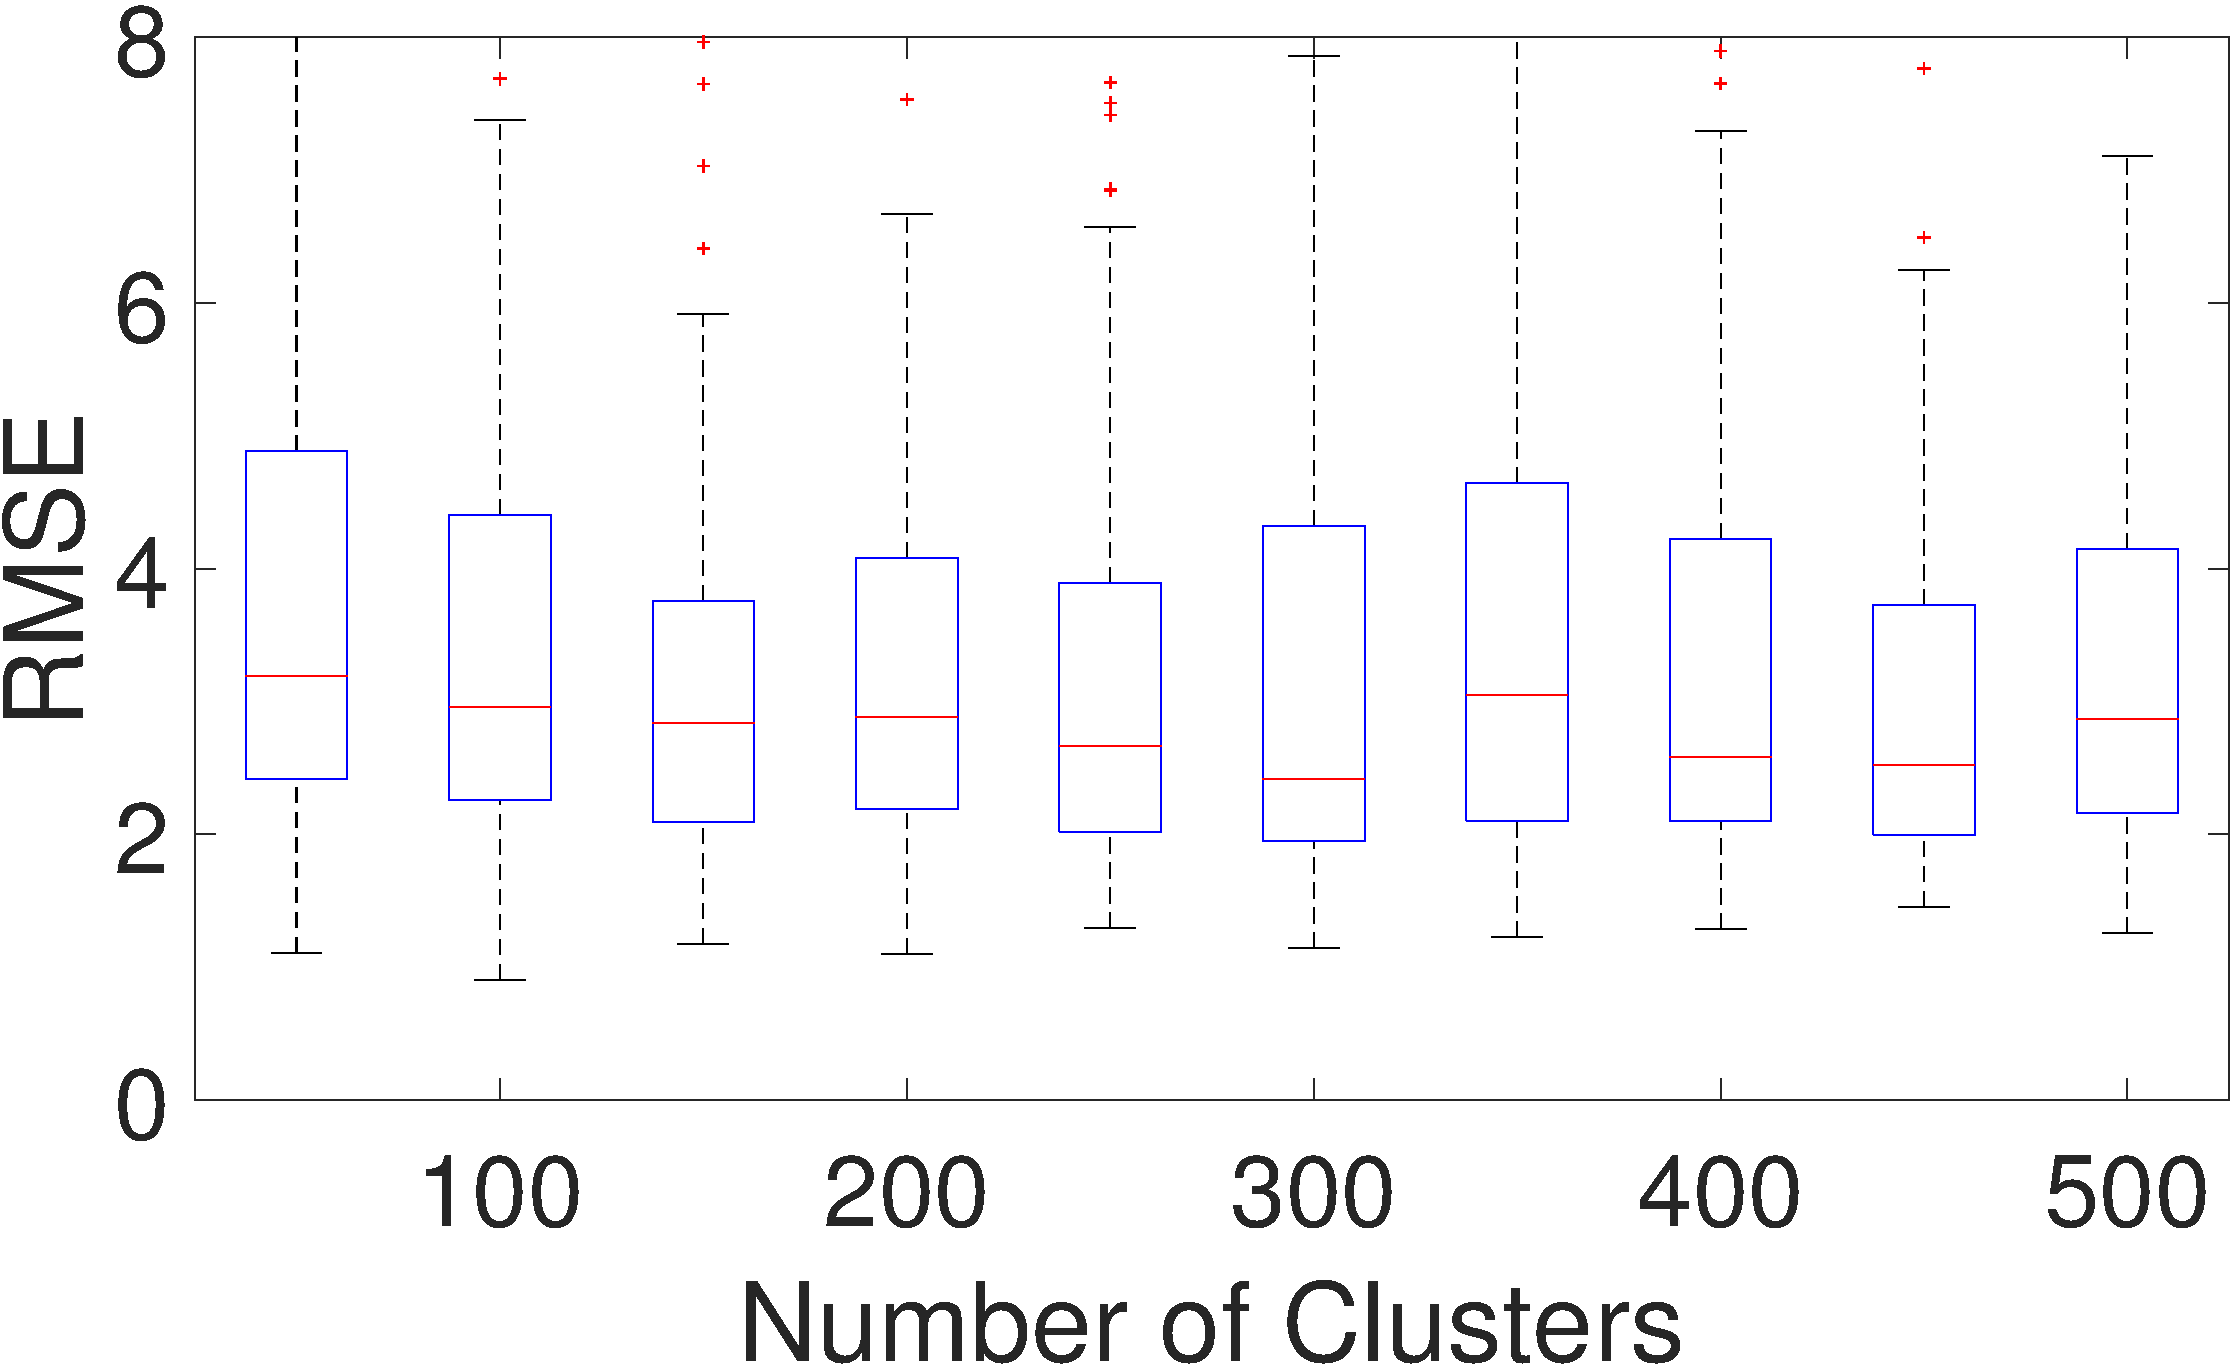
\includegraphics[width=0.3\textwidth]{Figures/RMSE_NbClusters_KNN5}}
%\subfigure[$K$=10]{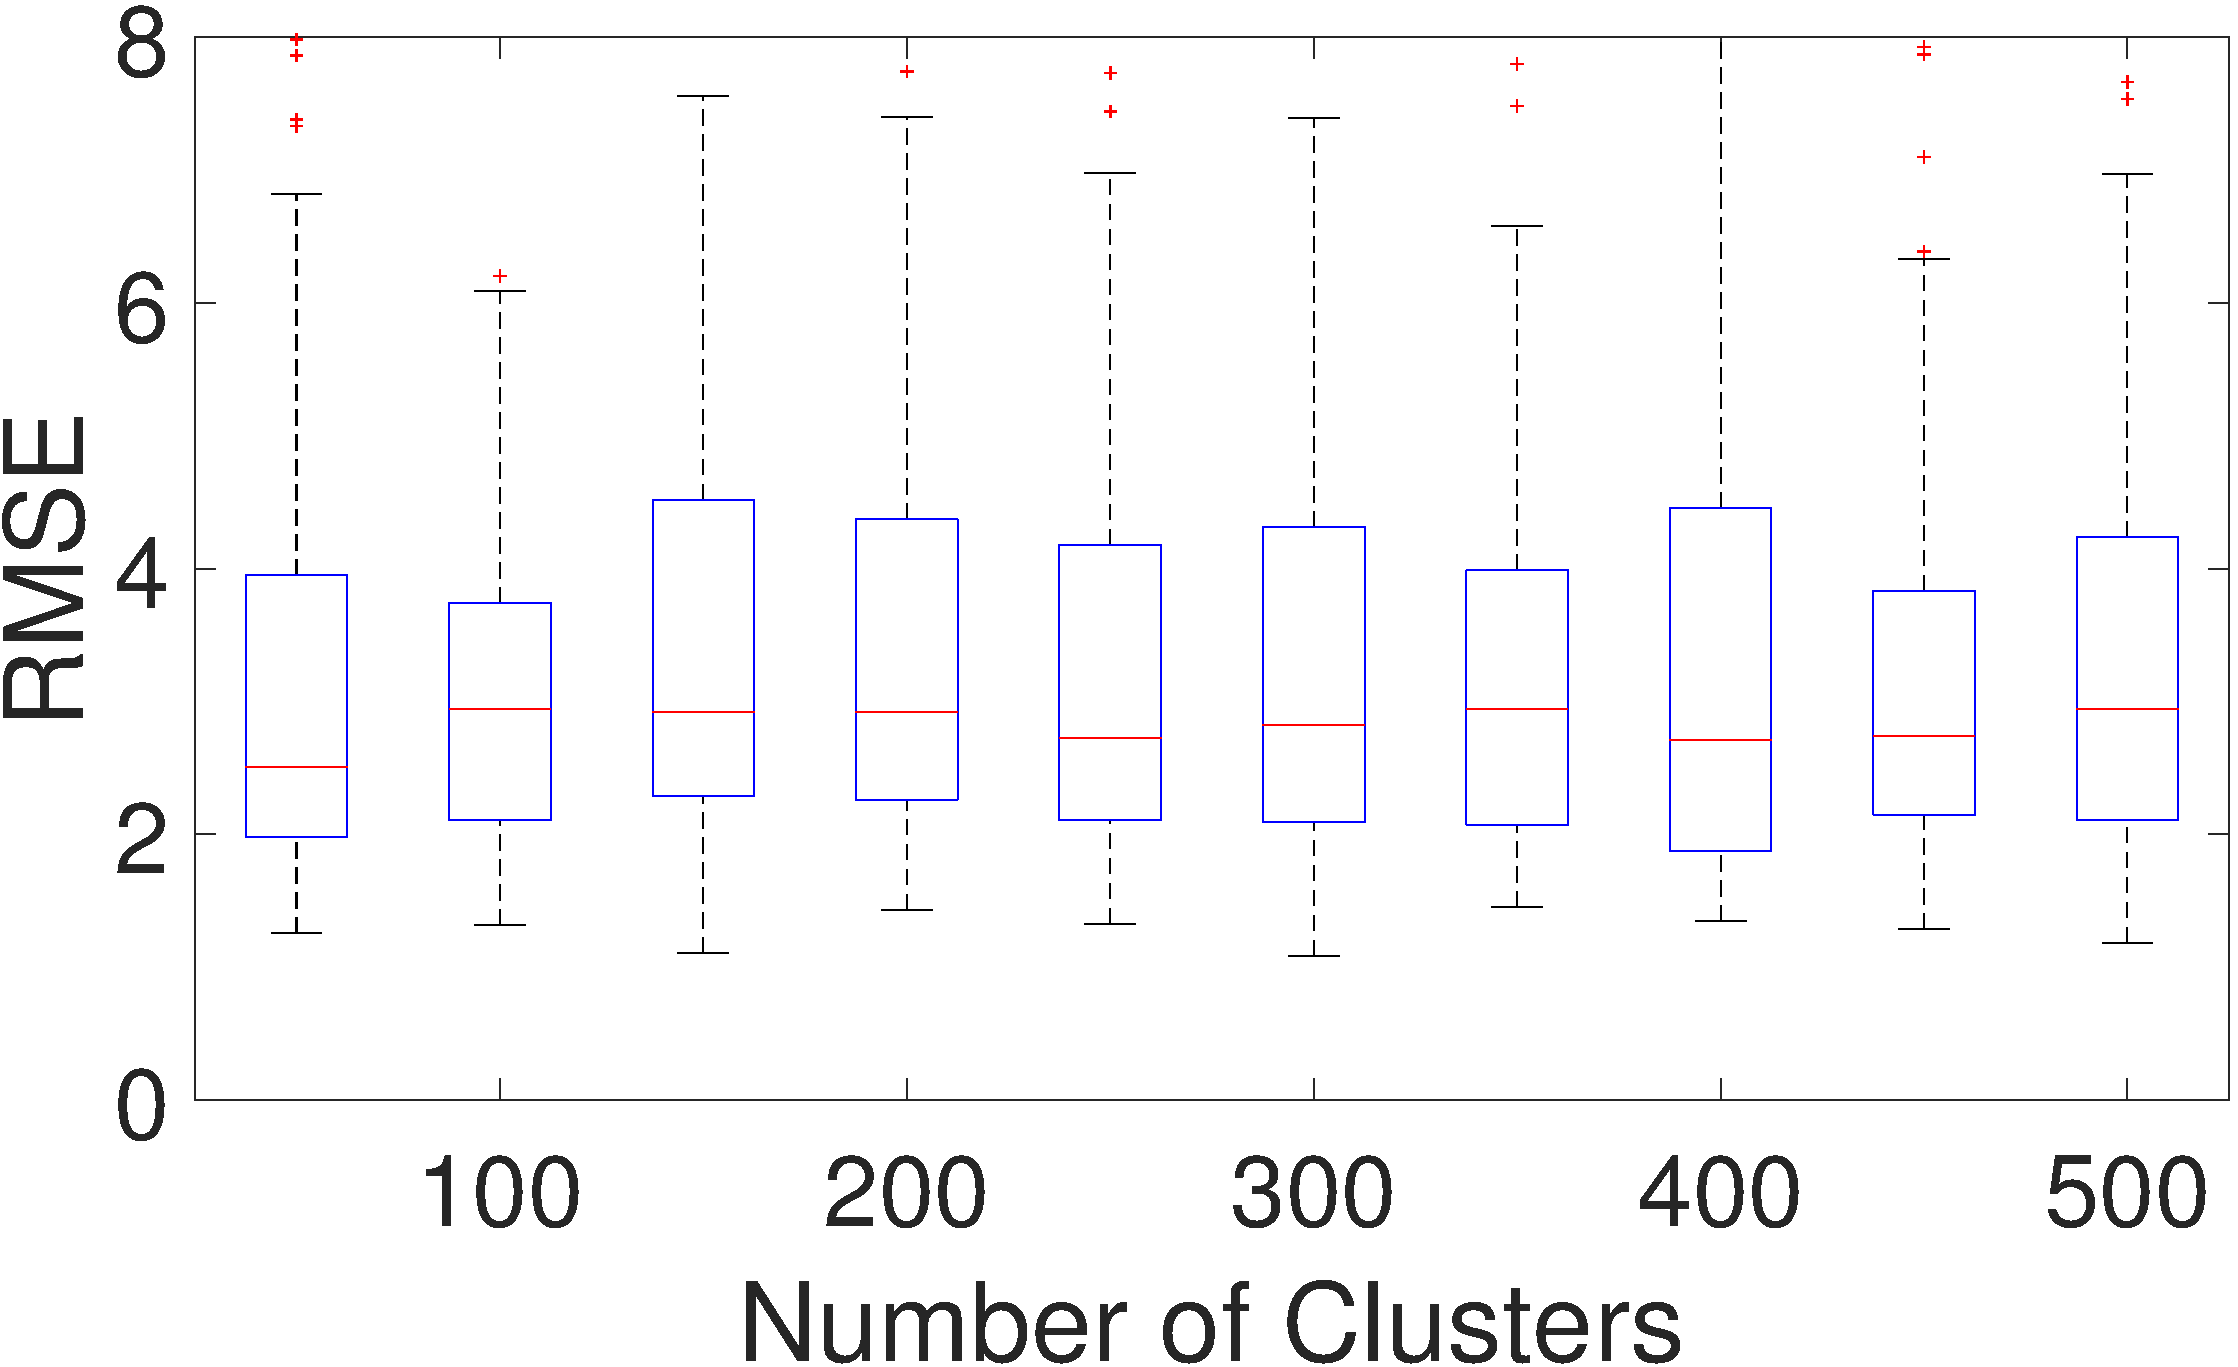
\includegraphics[width=0.3\textwidth]{Figures/RMSE_NbClusters_KNN10}}
%\subfigure[$K$=20]{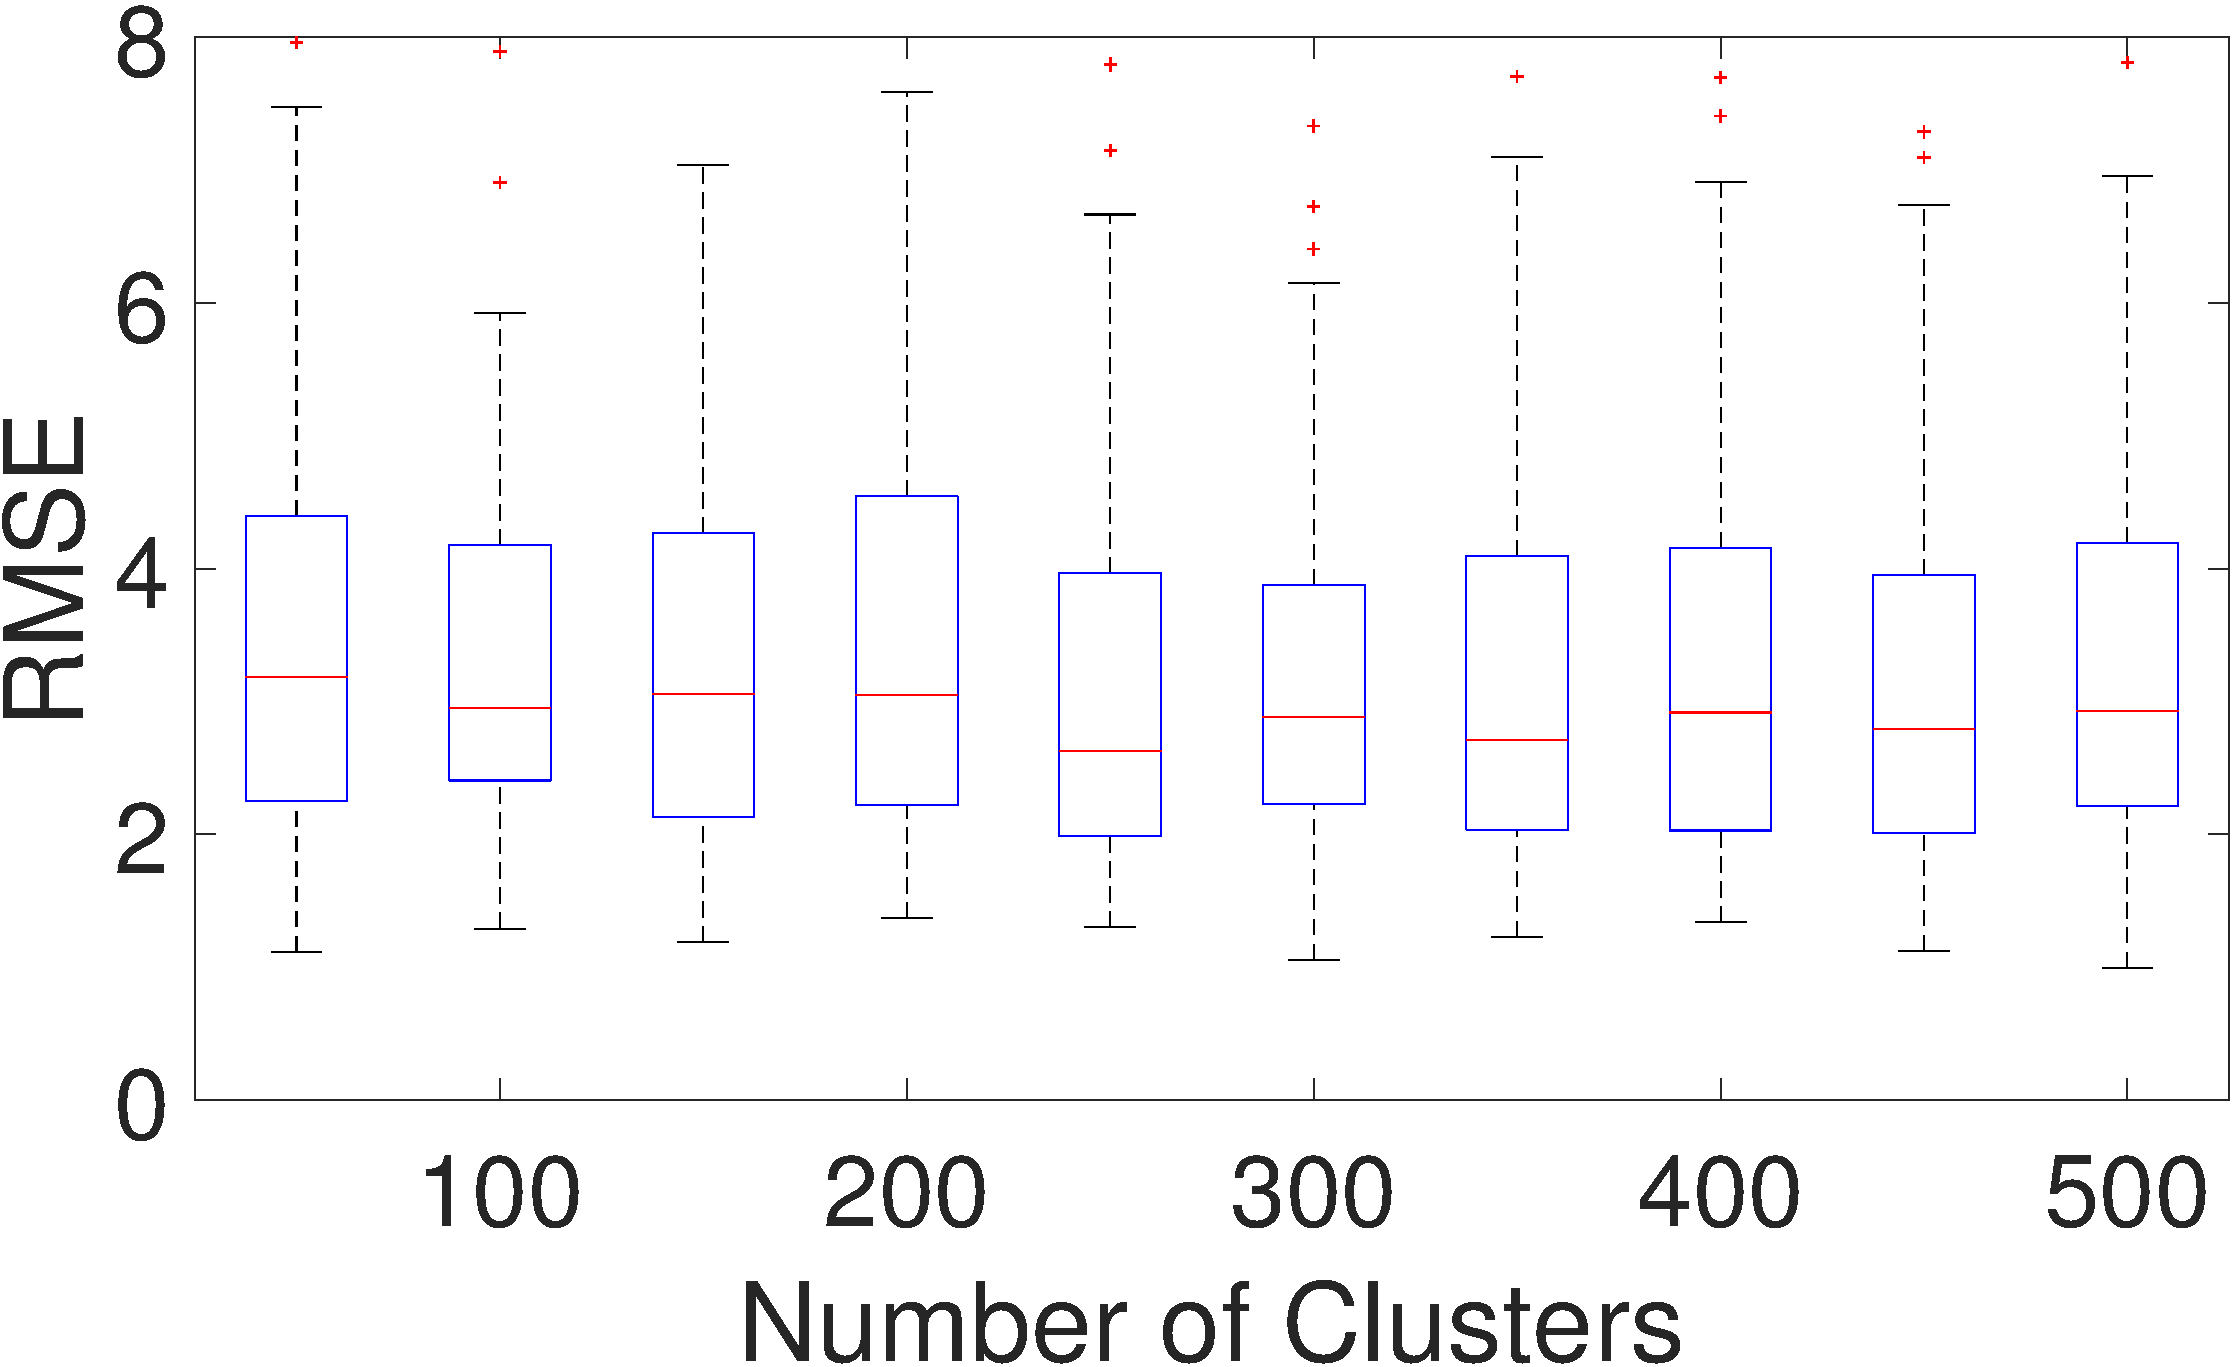
\includegraphics[width=0.3\textwidth]{Figures/RMSE_NbClusters_KNN20}}
%\caption{Boxplot of time-averaged RMSE of Clusterpf with respect to the number of eigenvectors over 100 Monte Carlo trials for different values of $K$.}
%\label{fig:RMSE_NbClusters}
%\end{figure}
%
%\begin{figure}
%\centering
%\subfigure[$K$=5]{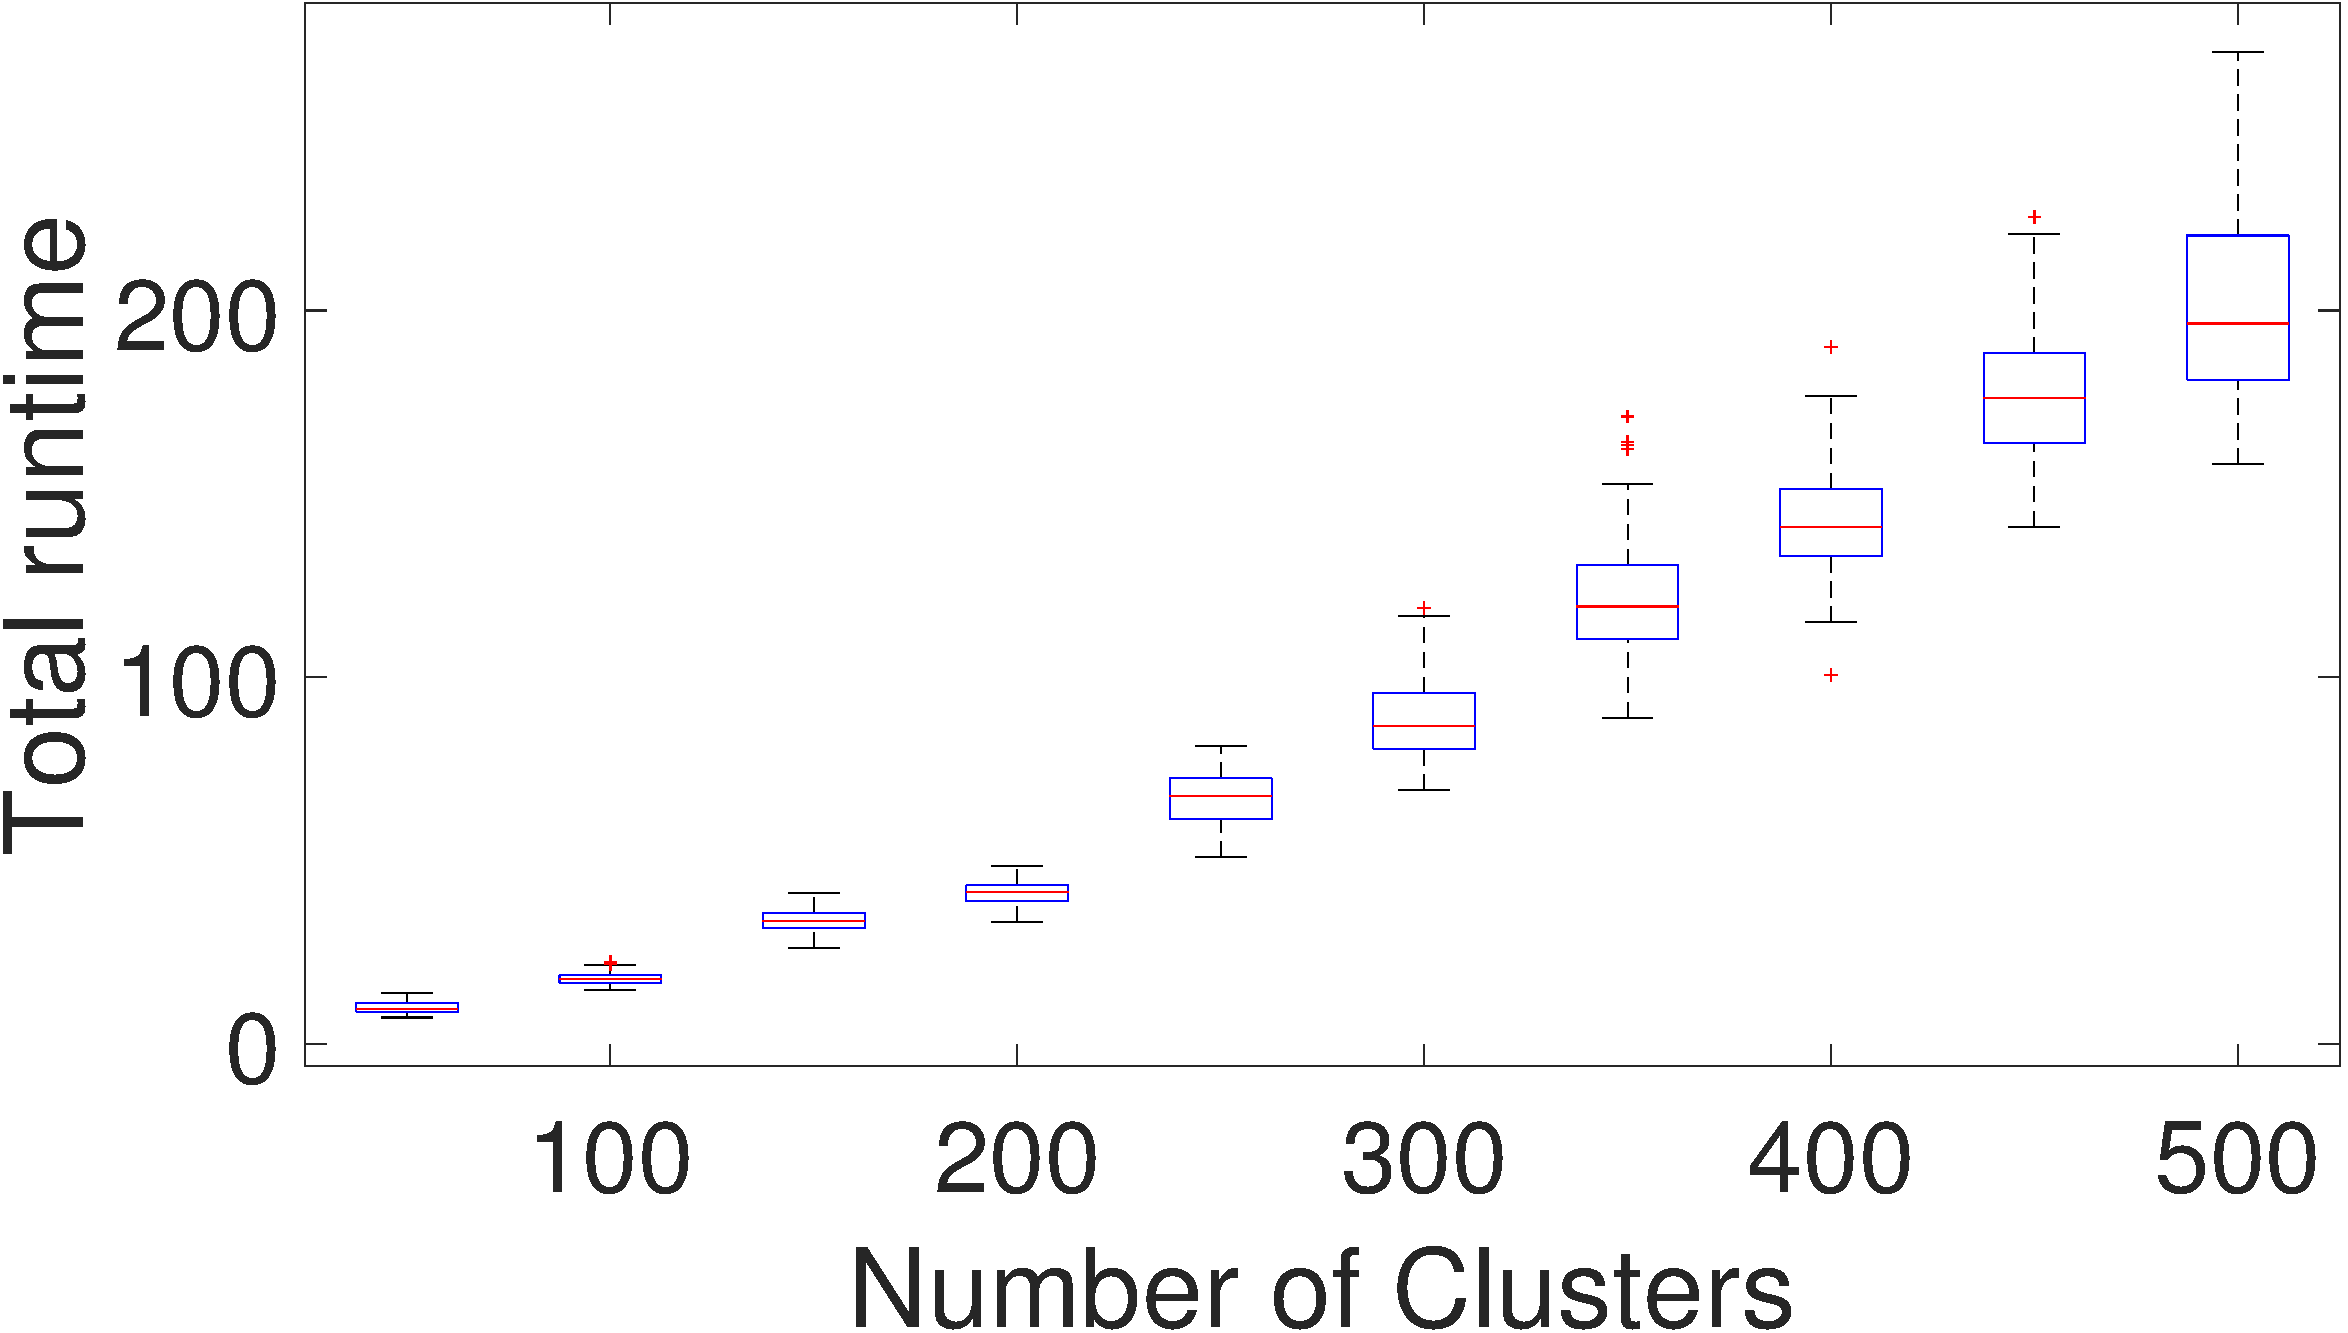
\includegraphics[width=0.3\textwidth]{Figures/runtime_NbClusters_KNN5}}
%\subfigure[$K$=10]{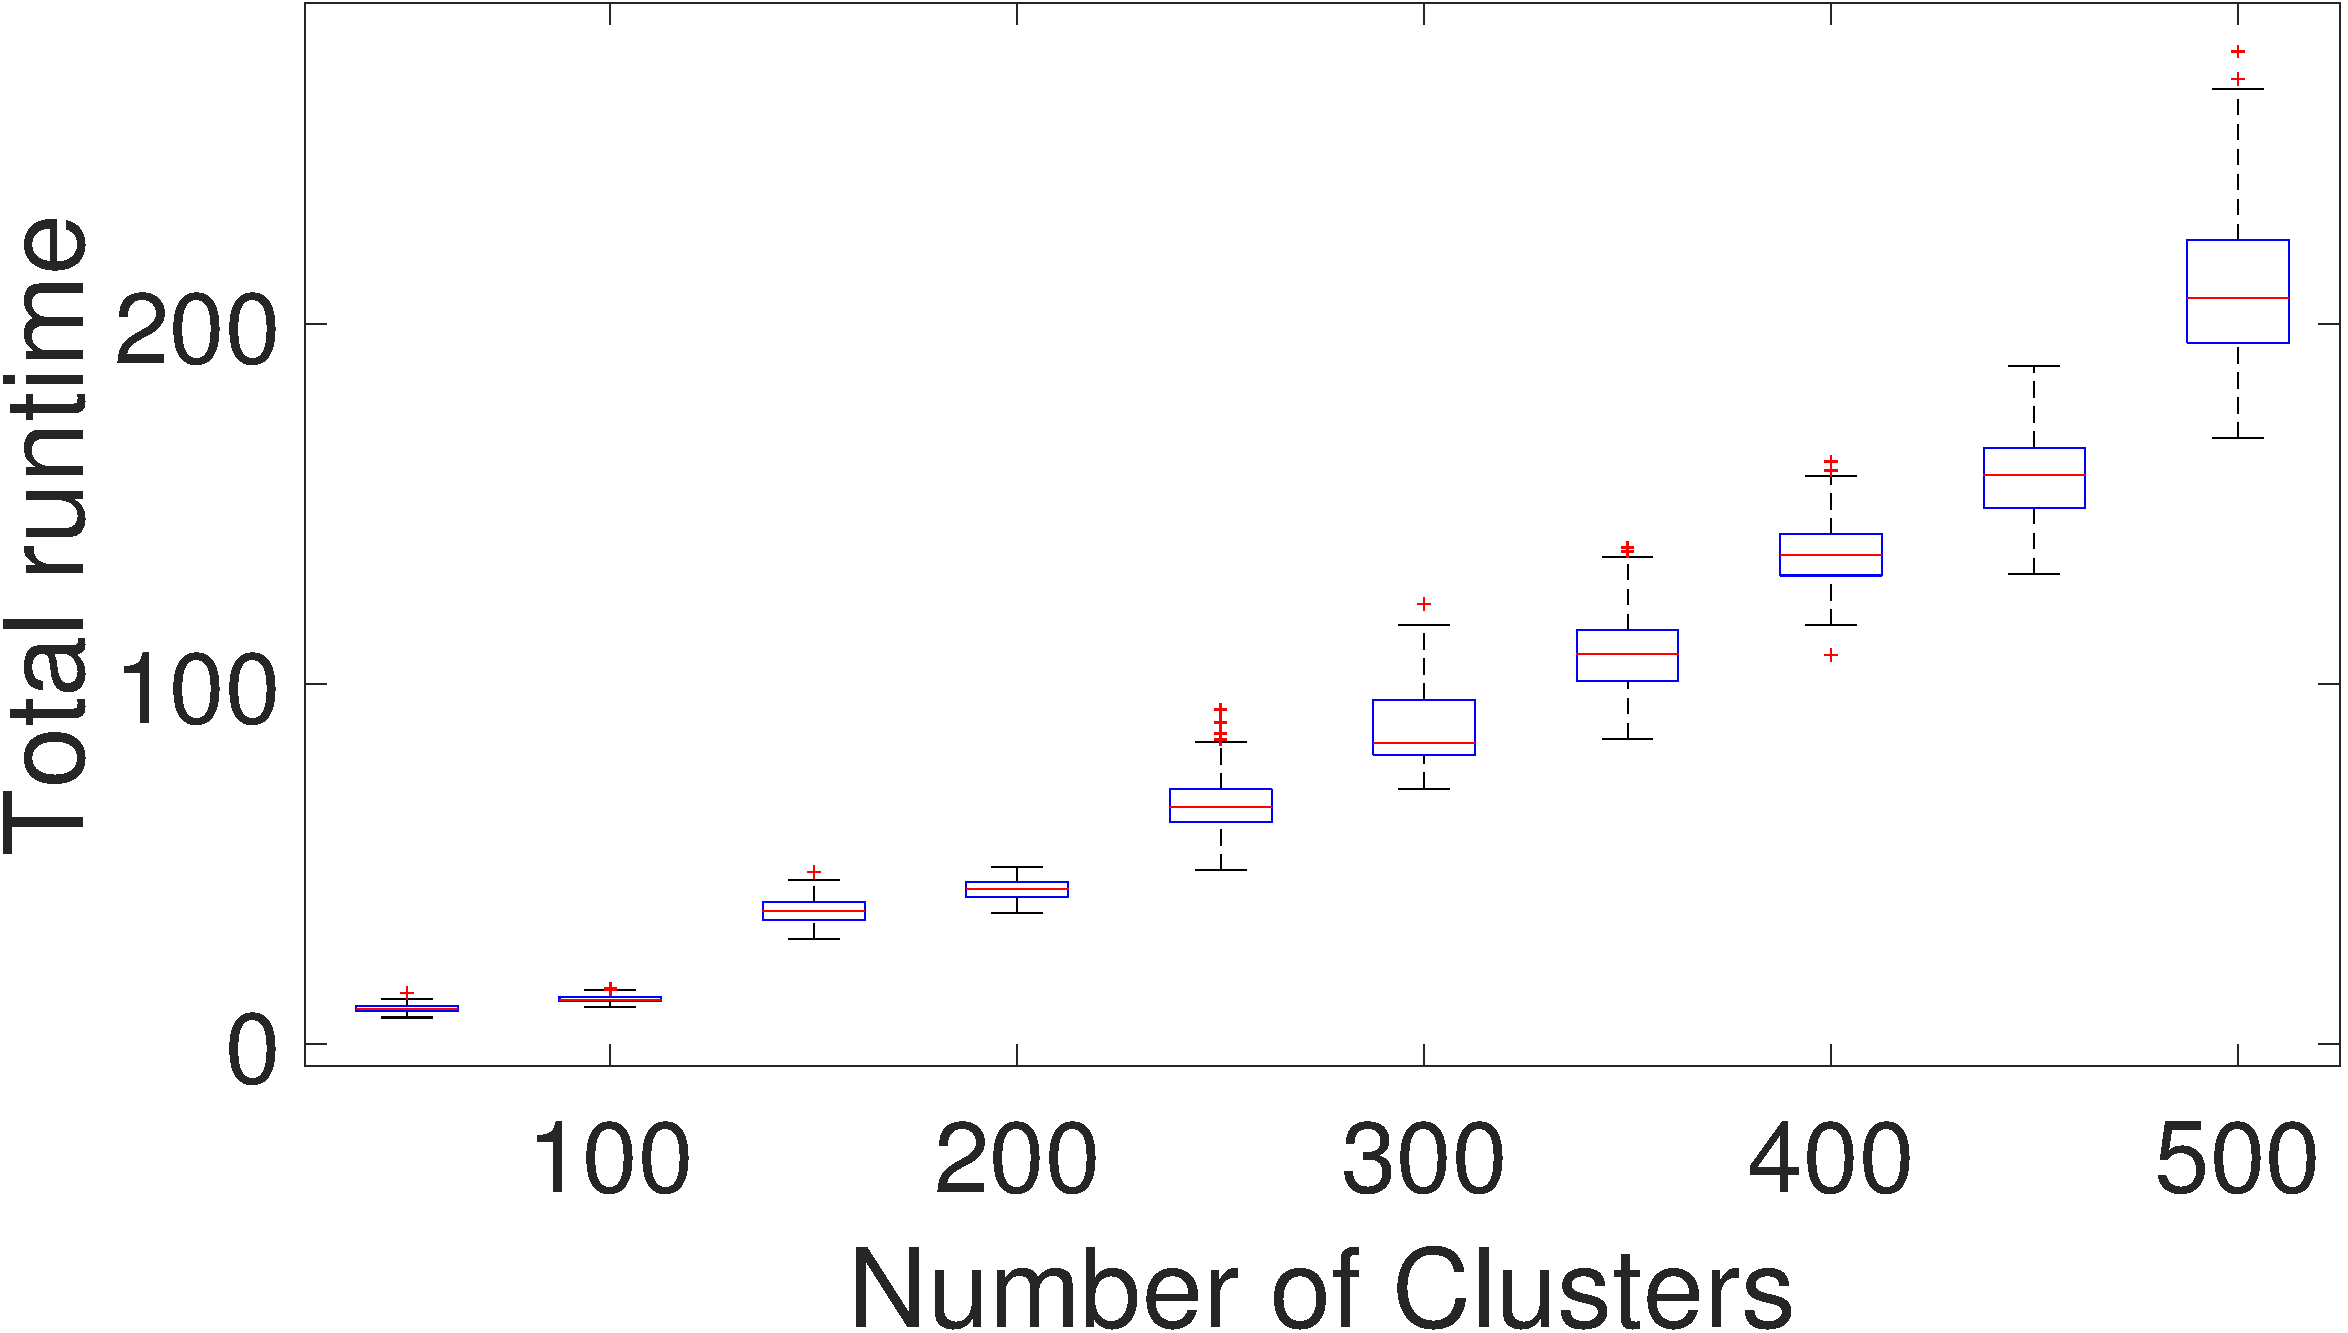
\includegraphics[width=0.3\textwidth]{Figures/runtime_NbClusters_KNN10}}
%\subfigure[$K$=20]{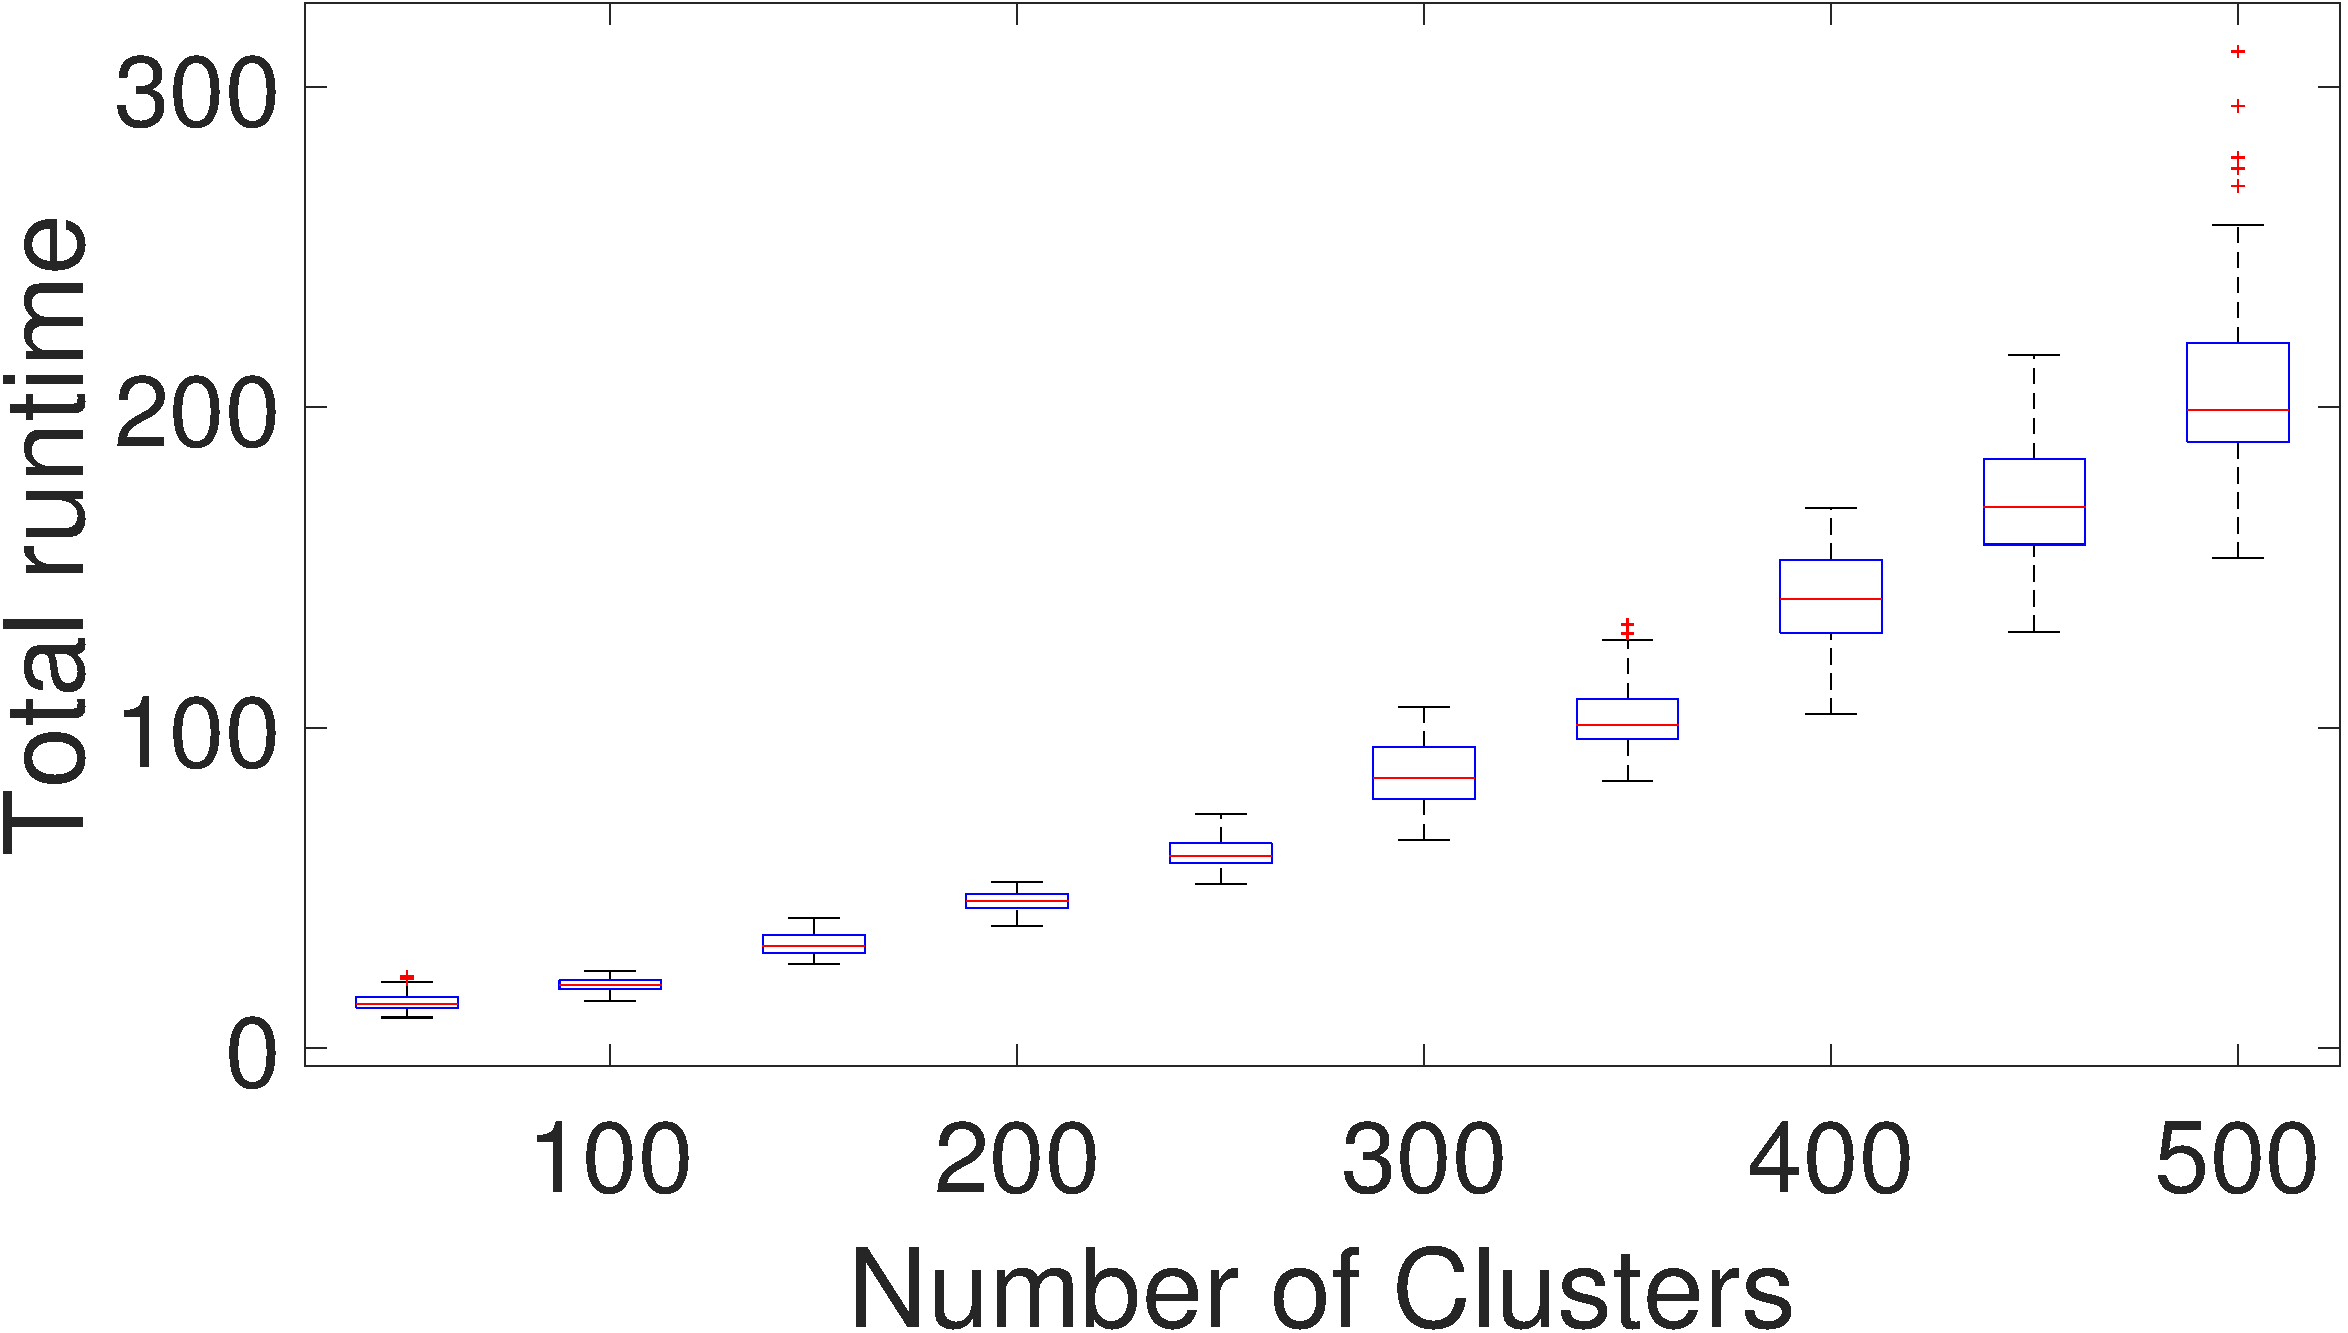
\includegraphics[width=0.3\textwidth]{Figures/runtime_NbClusters_KNN20}}
%\caption{Boxplot of total runtime of Clusterpf with respect to the number of eigenvectors over 100 Monte Carlo trials for different values of $K$.}
%\label{fig:runtime_NbClusters}
%\end{figure}
%

\subsection{Performance comparison between filters}
In this section, we compare the filters against each other. We consider a number of different tracks and investigate several parameters of interest. 

Fig.~\ref{fig:track1_results} shows the first test track and the boxplot of RMSE with respect to $N$, the number of particles. The CSSpf has the worst performance by a significant margin. For $N\geq 500$, the other four particle filters have similar performance. 

\begin{figure}
\centering
\begin{subfigure}[Track]
{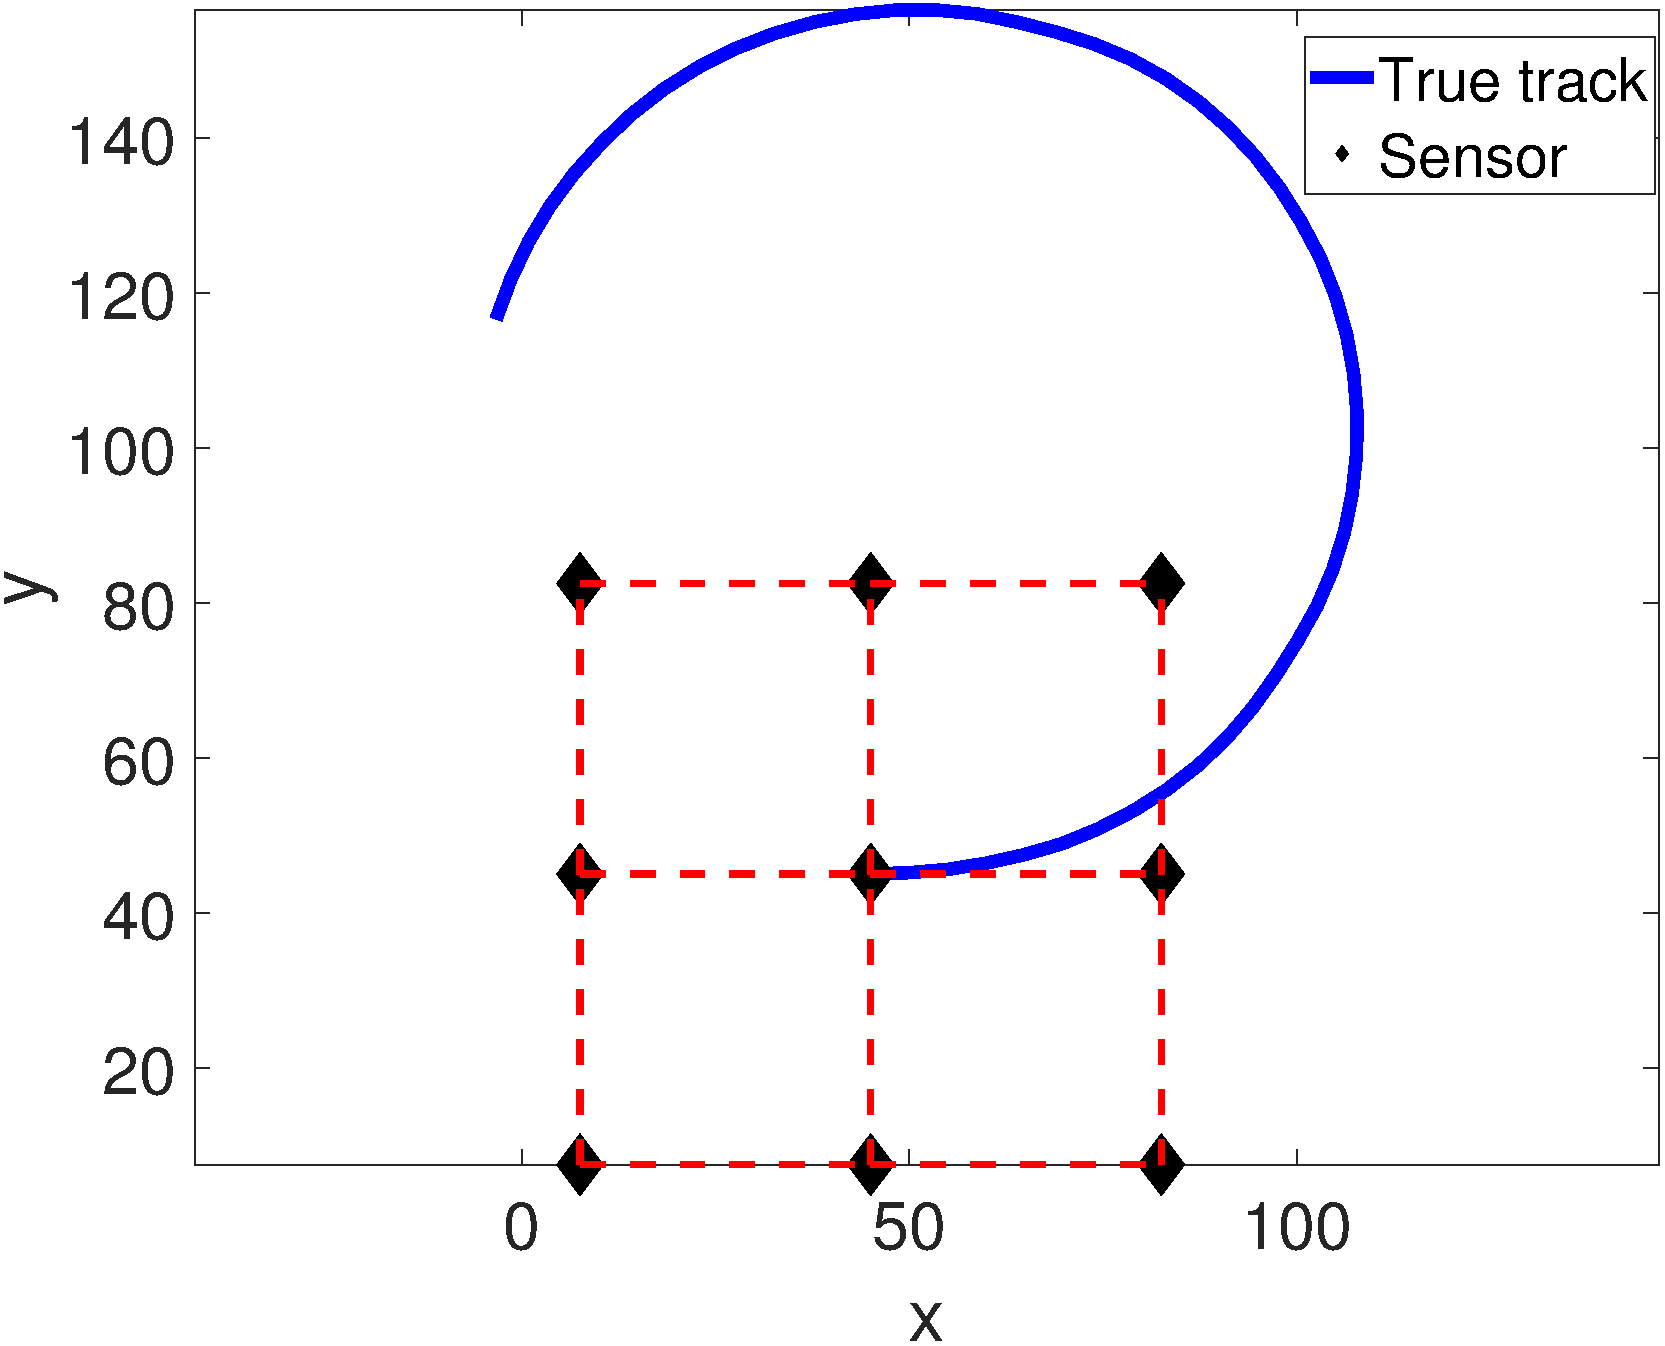
\includegraphics[width=0.45\textwidth]{Figures/track}}
\end{subfigure}
\begin{subfigure}[RMSE]
{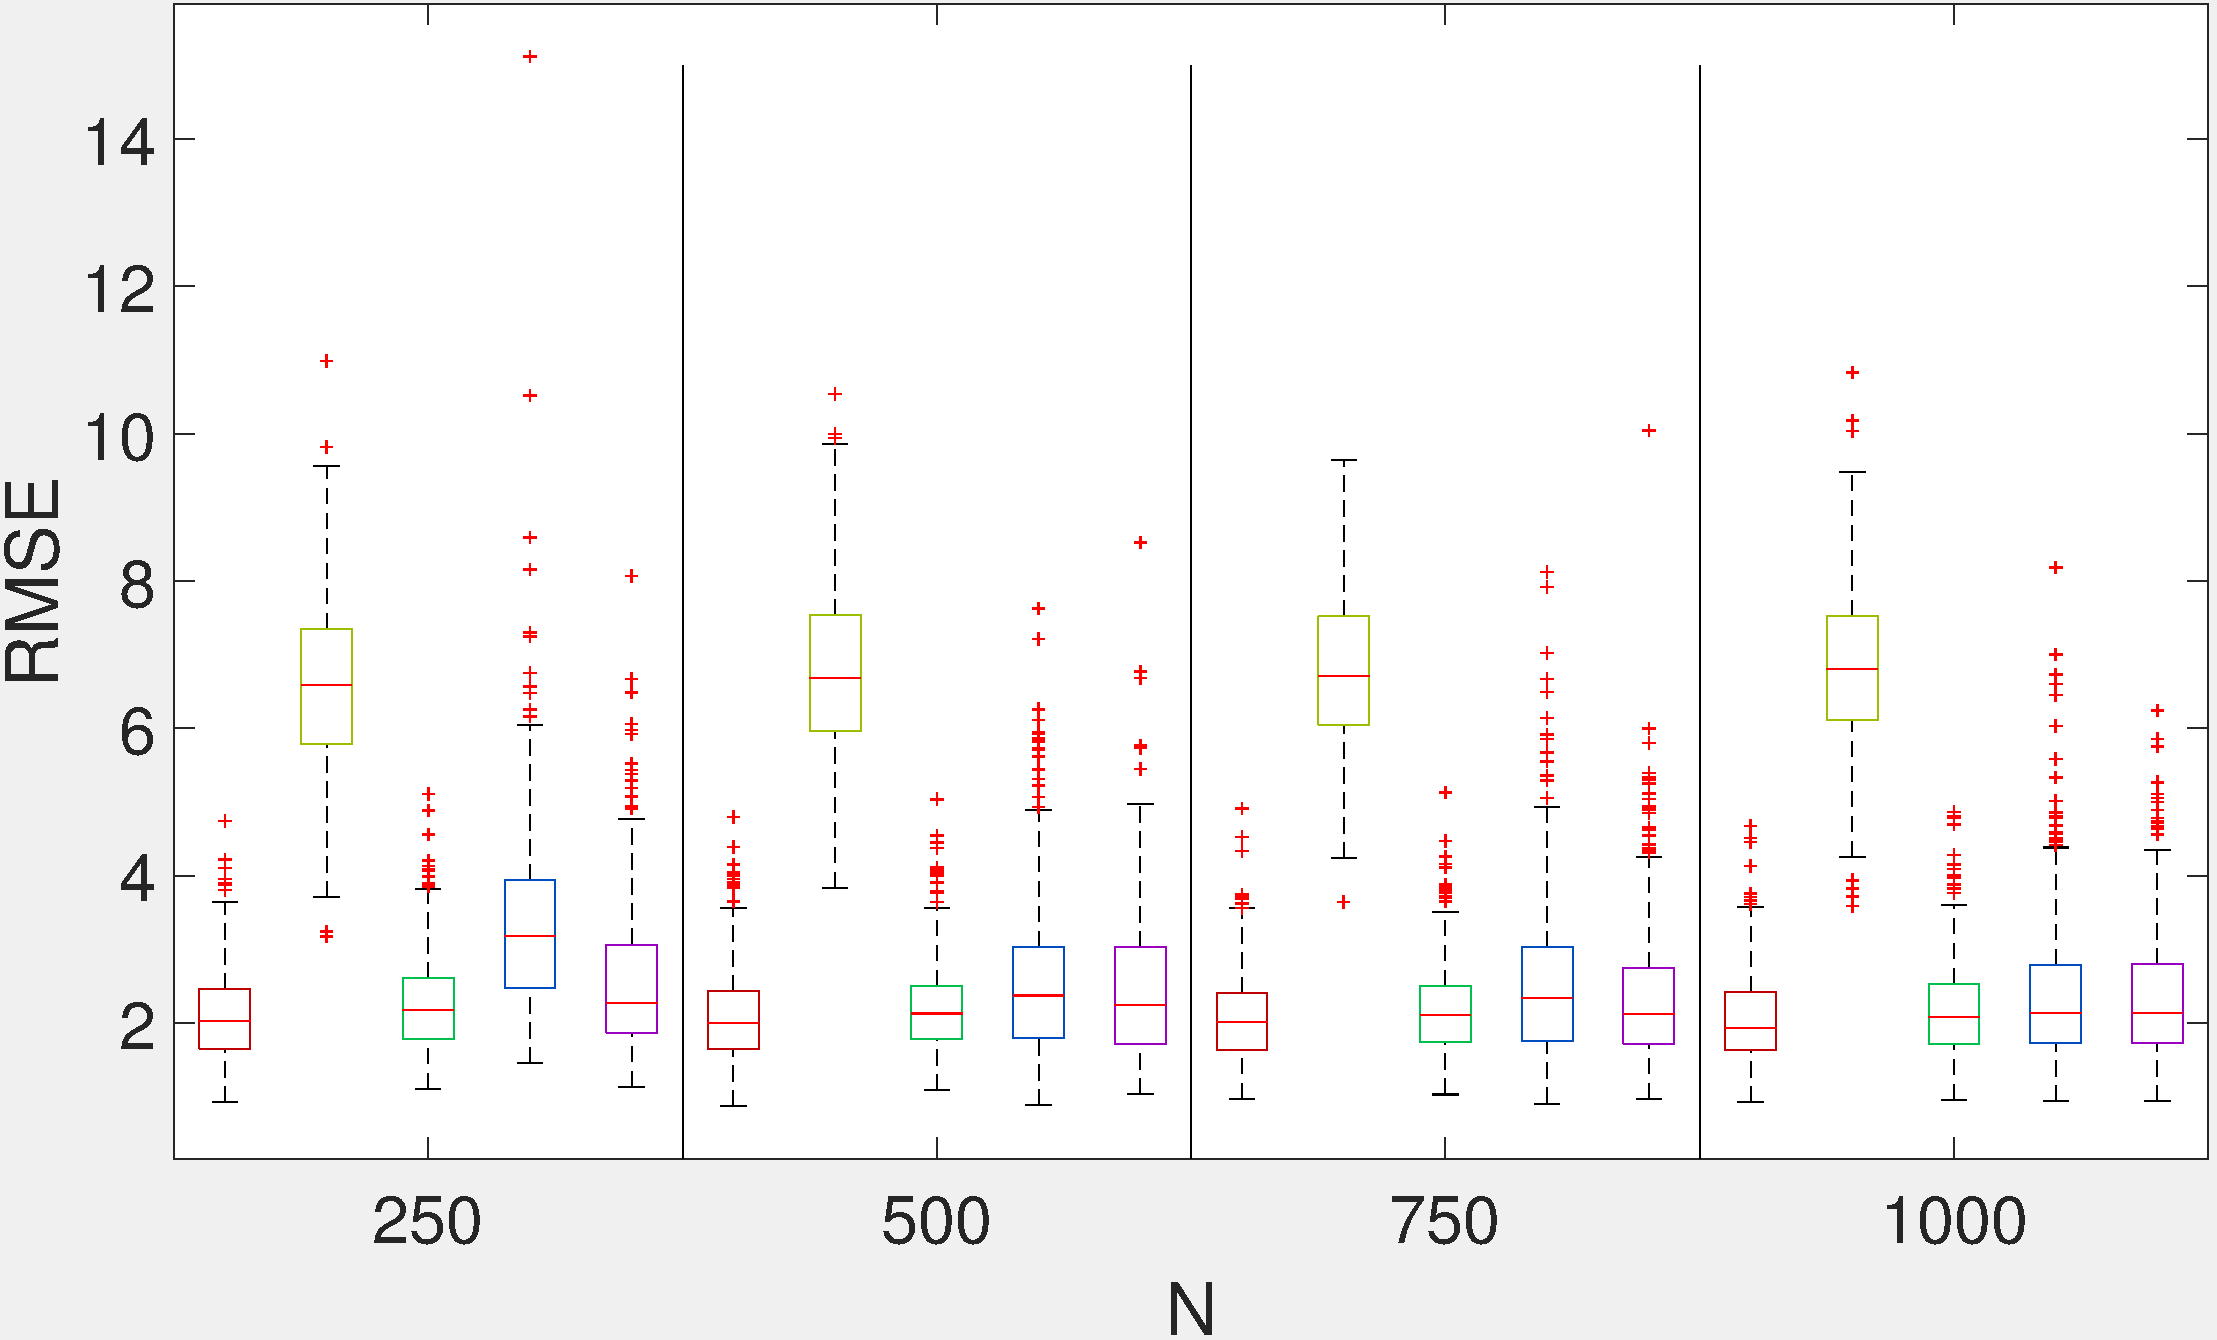
\includegraphics[width=0.45\textwidth]{Figures/RMSE_track1_N}}
\end{subfigure}
\caption{Test trajectory and boxplots of RMSE with respect to $N$. For each value of $N$, from left to right: BSpf, CSSpf, LCpf, LApf, Clusterpf}
\label{fig:track1_results}
\end{figure}

Next, we consider a different track that is completely outside the sensor grid. Fig.~\ref{fig:track2_results} shows the track and the results. Again, CSSpf has the worst performance by far. The other four filters have similar performance for $N\geq 500$; although the RMSE of LCpf has the largest fluctuation. 
\begin{figure}
\centering
\begin{subfigure}[Track]
{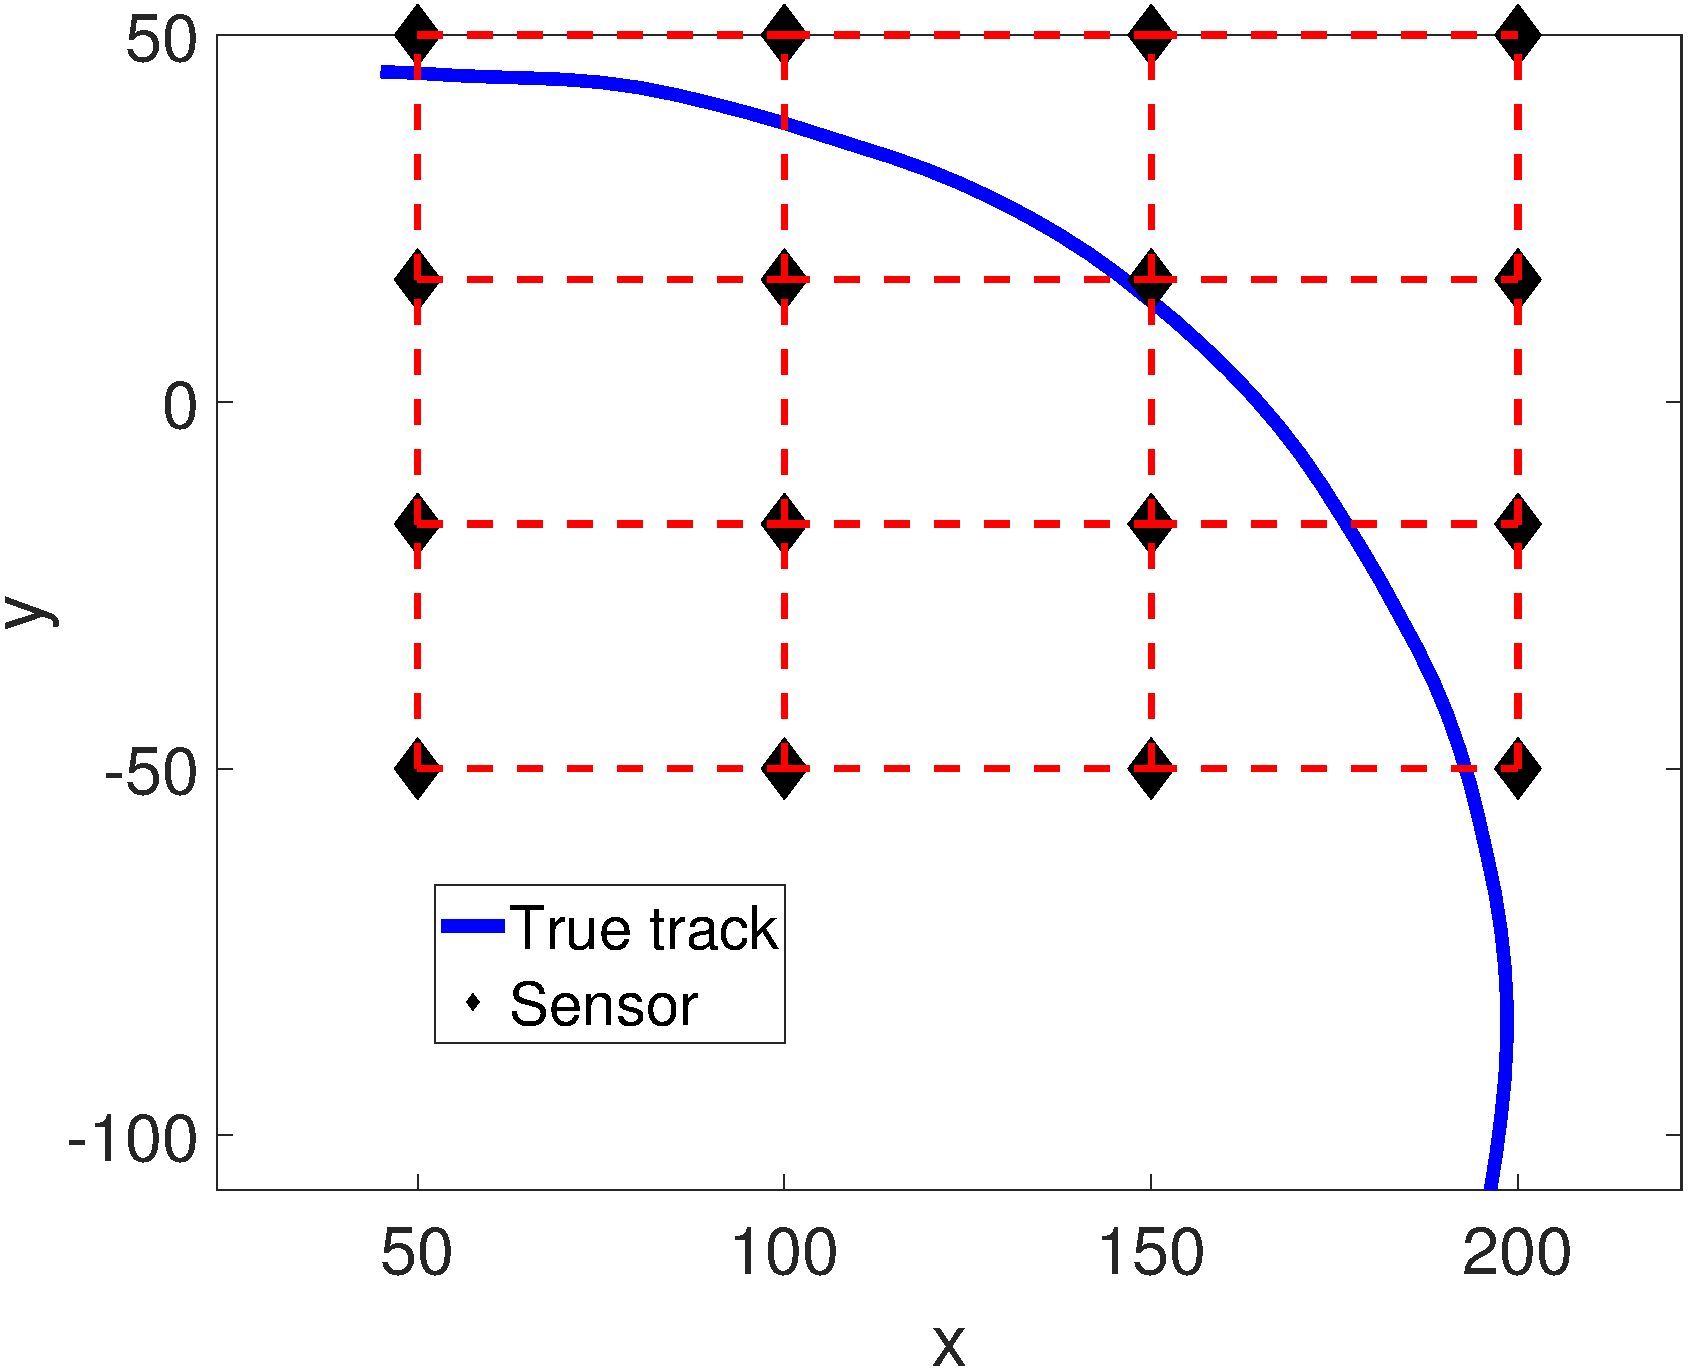
\includegraphics[width=0.45\textwidth]{Figures/track2}}
\end{subfigure}
\begin{subfigure}[RMSE]
{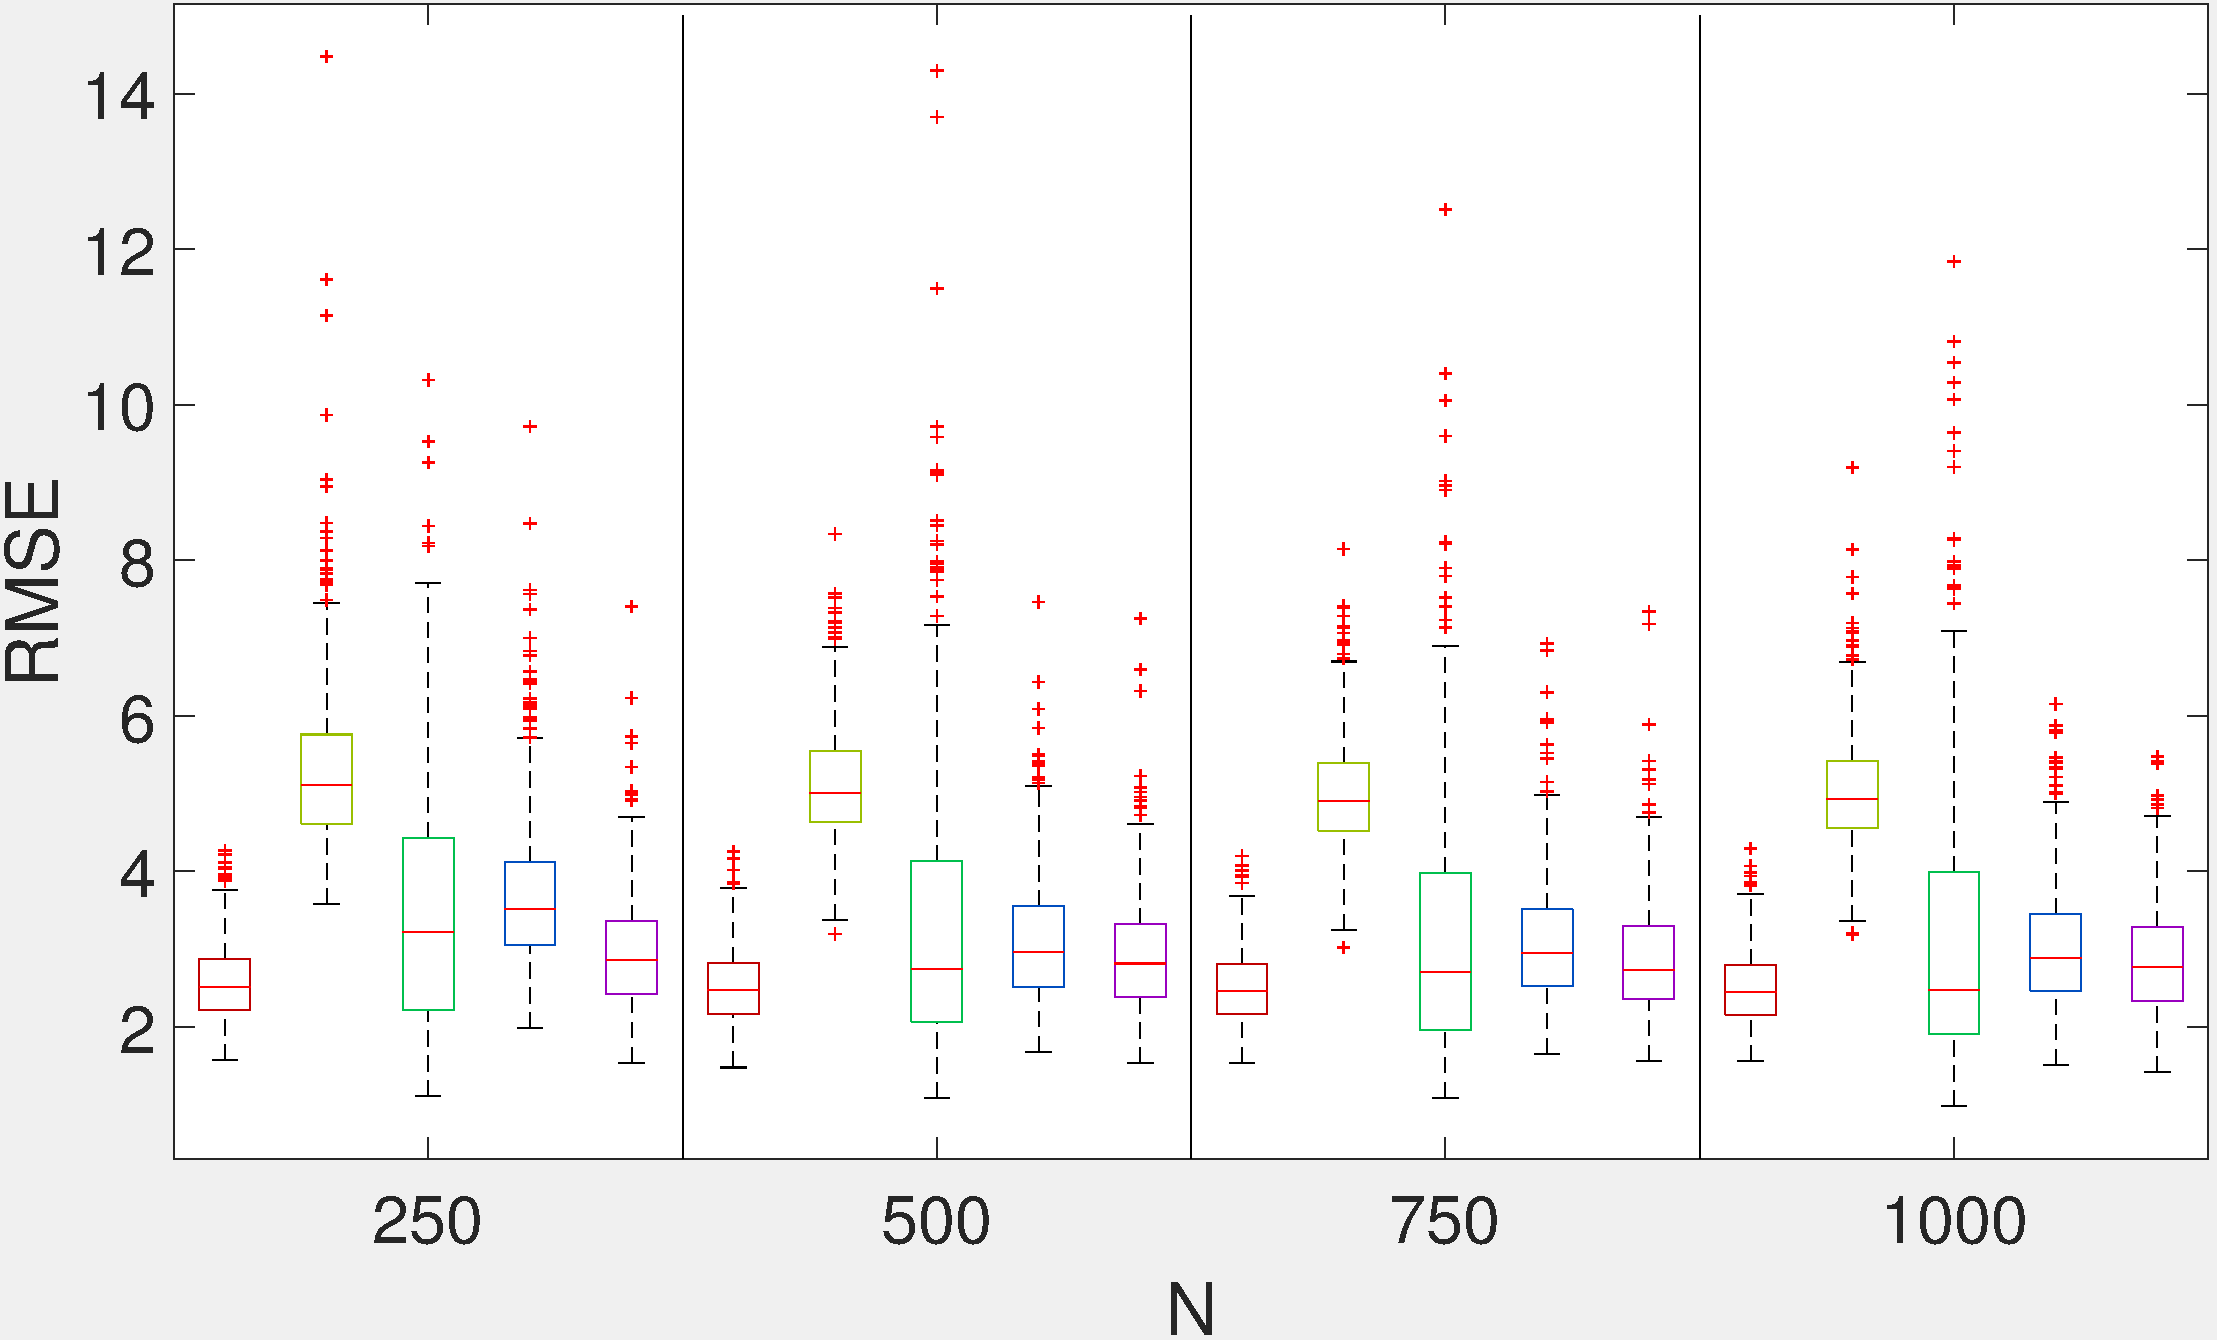
\includegraphics[width=0.45\textwidth]{Figures/RMSE_track2_N}}
\end{subfigure}
\caption{2nd Test trajectory and boxplots of RMSE with respect to $N$. For each value of $N$, from left to right: BSpf, CSSpf, LCpf, LApf, Clusterpf}
\label{fig:track2_results}
\end{figure}

In the third track, we expand the size of sensor grid to ensure that the target trajectory remains within the grid. 
\section{Conclusion}
\label{sec:conclusion}
To be completed

\end{document}
